\chapter{Who Creates Housing Bubbles? An Agent-Based Study}

\noindent\textbf{Citation:} Jiaqi Ge. (2014) Who Creates Housing Bubbles? An Agent-Based Study. \textit{Lecture Notes in Computer Science (including subseries Lecture Notes in Artificial Intelligence and Lecture Notes in Bioinformatics)}, 143-150. https://doi.org/10.1007/978-3-642-54783-6\_10

\vspace{0.5em}
\chapter{Exploring the Combined Effect of Factors Influencing Commuting Patterns and CO2 Emissions in Aberdeen Using an Agent-Based Model}

\noindent\textbf{Citation:} Jiaqi Ge; J Gary Polhill. (2016) Exploring the Combined Effect of Factors Influencing Commuting Patterns and CO2 Emissions in Aberdeen Using an Agent-Based Model. \textit{Journal of Artificial Societies and Social Simulation}, 19(3). https://doi.org/10.18564/jasss.3078

\noindent\textbf{Abstract}\par
\begin{quote}\small
This paper develops an agent-based model of the daily commute in Aberdeen City and the surrounding area in Scotland, UK. We study the impact of flexitime work arrangements, urban concentration, a new bypass, and cycle lanes on commute time length, reliability and CO2 emissions, and analyse the diverse conflation of these factors and the different connections of them in order to detect their cumulative effects. Our results suggest that flexitime will reduce CO2 emissions from traffic. It also reduces mean commute time and makes commute time more reliable. We find that although higher urban concentration will make travel time less reliable, it will reduce CO2 emissions from commuting and cut commute time length. There might also be a trade-off between travel time length and reliability regarding urban concentration. We show that the new bypass will only reduce mean commute time by a small amount, while slightly increasing total CO2 emissions. Finally, we find that cyclists sharing roads with cars do not necessarily slow down the traffic on the whole. We conclude that infrastructural, social and urban issues should never be studied in isolation with each other, and that urban policies will have ramifications for both urban and surrounding ex-urban areas.
\end{quote}

\vspace{0.5em}
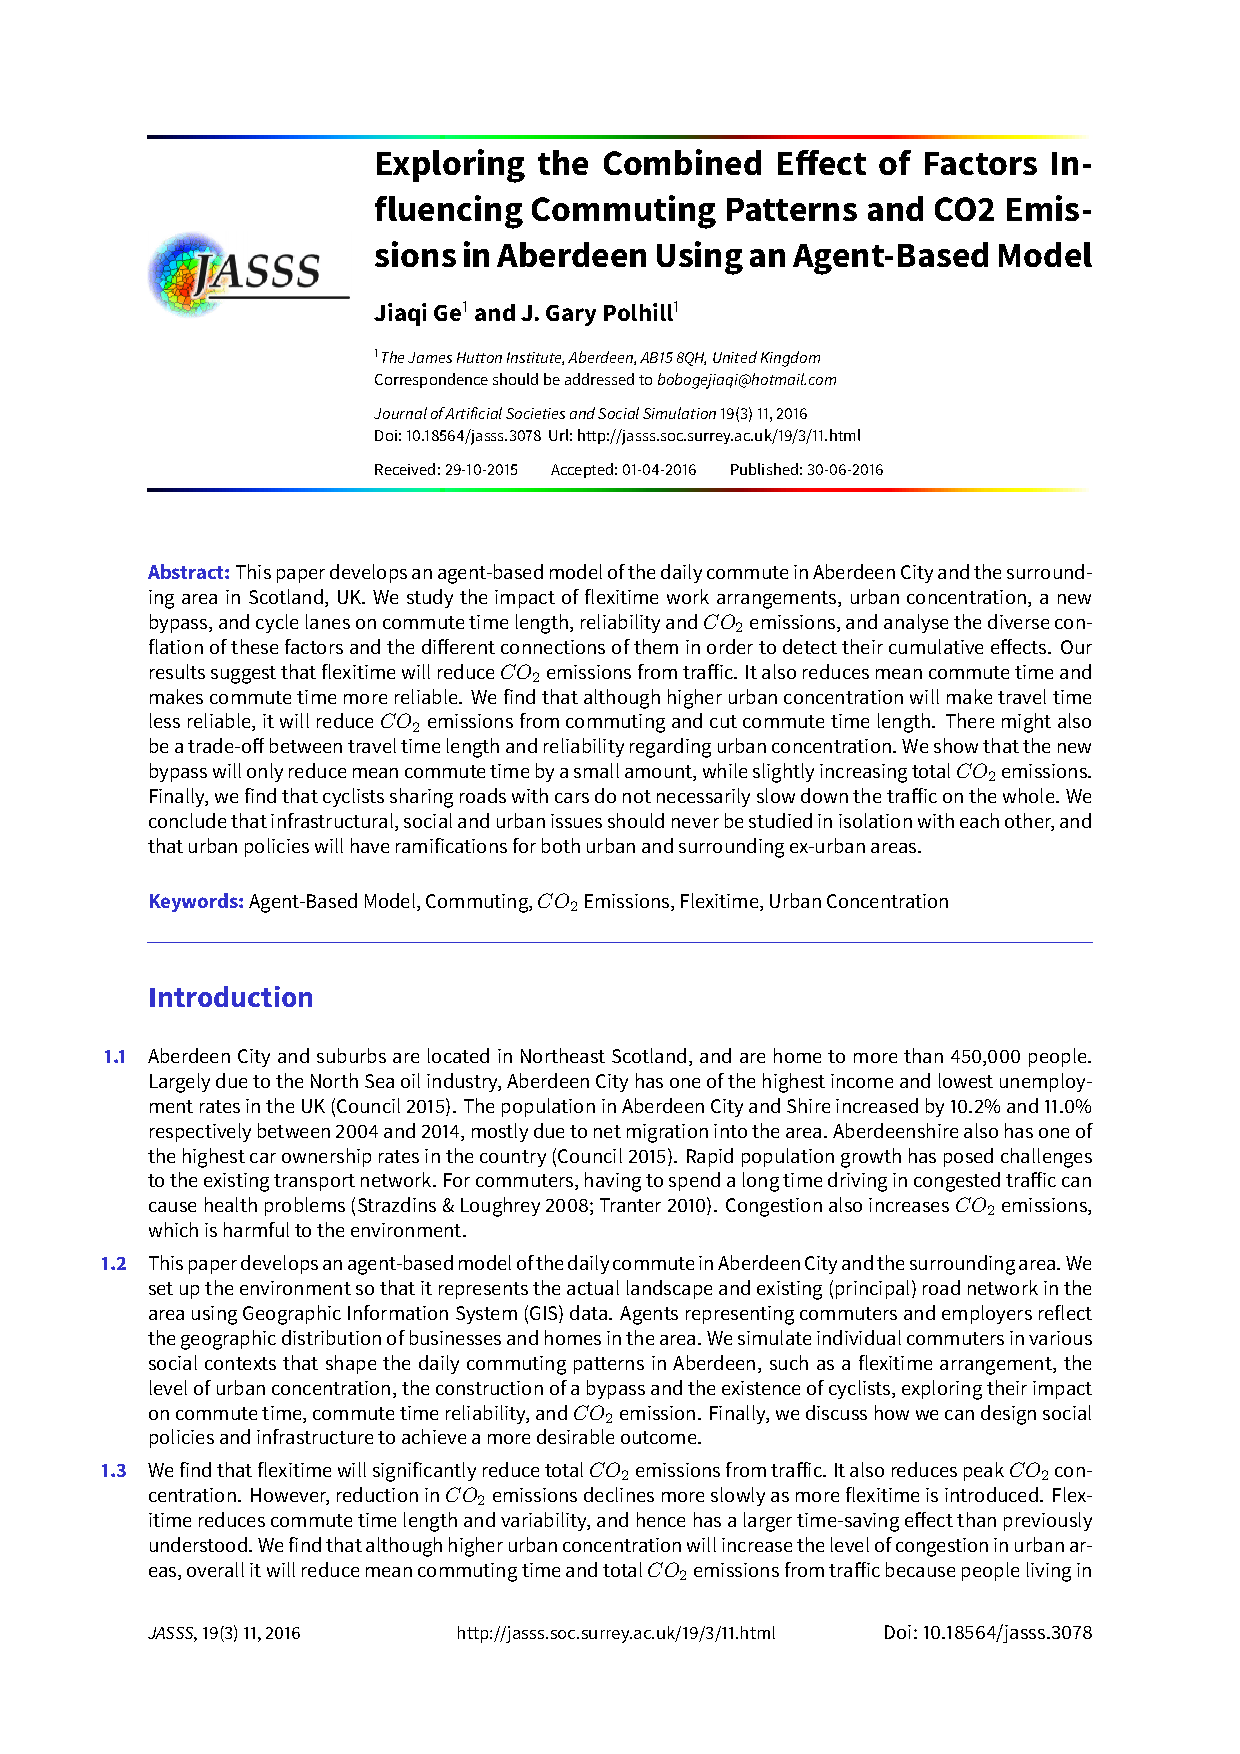
\includepdf[pages=-]{pdfs/10.18564_jasss.3078.pdf}

\chapter{Preliminary Results from an Agent-Based Model of the Daily Commute in Aberdeen and Aberdeenshire, UK}

\noindent\textbf{Citation:} J Ge; G Polhill. (2017) Preliminary Results from an Agent-Based Model of the Daily Commute in Aberdeen and Aberdeenshire, UK. \textit{Advances in Soft Computing}, 129-142. https://doi.org/10.1007/978-3-319-47253-9\_11

\vspace{0.5em}
\chapter{Endogenous rise and collapse of housing price: An agent-based model of the housing market}

\noindent\textbf{Citation:} Jiaqi Ge. (2017) Endogenous rise and collapse of housing price: An agent-based model of the housing market. \textit{Computers, Environment and Urban Systems}, 62, 182-198. https://doi.org/10.1016/j.compenvurbsys.2016.11.005

\noindent\textbf{Abstract}\par
\begin{quote}\small
On the basis of interviews with local real estate agents, this study develops an agent-based model of housing market to determine the cause of rise and collapse of US housing price during the years immediately preceding the US financial crisis (2007-2009). We study the key factors affecting housing price volatility, such as lenient financing and speculation. The dynamic simulation findings in the study show in concrete terms how lenient lending practices combined with speculation can lead to increased volatility in housing price, including sharp rises immediately followed by collapses. The exploratory work in this study will contribute to the understanding of the causes of housing bubbles and inform policy decisions.
\end{quote}

\vspace{0.5em}
\chapter{Exploring factors affecting on-farm renewable energy adoption in Scotland using large-scale microdata}

\noindent\textbf{Citation:} Jiaqi Ge; Lee-Ann Sutherland; J Gary Polhill; Keith Matthews; Dave Miller; Douglas Wardell-Johnson. (2017) Exploring factors affecting on-farm renewable energy adoption in Scotland using large-scale microdata. \textit{Energy Policy}, 107, 548-560. https://doi.org/10.1016/j.enpol.2017.05.025

\noindent\textbf{Abstract}\par
\begin{quote}\small
This paper uses large-scale micro data to identify key factors affecting the decision to adopt renewable energy generation (wind, solar and biomass) on farms in Scotland. We construct an integrated dataset that includes the compulsory agricultural census and farm structural survey that cover almost all farms in Scotland. In addition to farm owner demographics and farm business structures, we also assess the effect of diversification activities such as tourism and forestry, as well as the spatial, biophysical and geophysical attributes of the farms on the adoption decision. We find that diversified farms are more likely to adopt renewable energy, especially solar and biomass energy. Farms are also more likely to adopt renewable energy if they have high local demand for energy, or suitable conditions for renewable energy production. We find that biophysical factors such as the agricultural potential of farm land are important in adoption decisions. We identify adopter profiles for each type of renewable energy, and map the geographic location of potential adopters. We argue that renewable energy policy should be more integrated with farm diversification policy and farm support schemes. It should also be tailored for each type of renewable energy, for the potential adopter profiles of wind, solar and biomass energy all differ in farm characteristics and geographic distribution.
\end{quote}

\vspace{0.5em}
\chapter{Does Work-life Balance Affect Pro-environmental Behaviour? Evidence for the UK Using Longitudinal Microdata}

\noindent\textbf{Citation:} Patricia C Melo; Jiaqi Ge; Tony Craig; Mark J Brewer; Ines Thronicker. (2018) Does Work-life Balance Affect Pro-environmental Behaviour? Evidence for the UK Using Longitudinal Microdata. \textit{Ecological Economics}, 145, 170-181. https://doi.org/10.1016/j.ecolecon.2017.09.006

\noindent\textbf{Abstract}\par
\begin{quote}\small
The environmental challenges we face today have made the need to behave pro-environmentally increasingly salient. Many believe that the modern day “busyness” of life and lack of spare time have kept people from acting according to their values and behaving more pro-environmentally. This study uses microdata from the UK Household Longitudinal Study (UKHLS) to investigate the relation between pro-environmental behaviour, environmental self-perception and work-life balance. Pro-environmental behaviour covers 21 behaviours relating to home energy, personal transport, recycling and shopping. Work-life balance is defined with relation to the availability of discretionary time using both objective and subjective measures. The results from the regression models of overall pro-environmental behaviour suggest that work-life imbalance does not appear to affect, neither directly nor indirectly through environmental values and attitudes, pro-environmental behaviour. The main factors determining the extent of pro-environmental behaviour relate to individual's attitudes towards the environment, age, educational attainment, household income and the presence of young children. The sensitivity analysis looking at differing time demanding behaviours reveals that actual availability of discretionary time does not seem to affect pro-environmental behaviour, while the subjective experience of work-life imbalance can have a negative direct effect particularly for more time demanding pro-environmental behaviours.
\end{quote}

\vspace{0.5em}
\chapter{Too much of a good thing? Using a spatial agent-based model to evaluate “unconventional” workplace sharing programmes}

\noindent\textbf{Citation:} Jiaqi Ge; J Gareth Polhill; Tony P Craig. (2018) Too much of a good thing? Using a spatial agent-based model to evaluate “unconventional” workplace sharing programmes. \textit{Journal of Transport Geography}, 69, 83-97. https://doi.org/10.1016/j.jtrangeo.2018.04.005

\noindent\textbf{Abstract}\par
\begin{quote}\small
Using a spatial agent-based model of transport, this paper explores various "unconventional" workplace sharing programmes that allow employees to work remotely at other work sites in Northeast Scotland, with Aberdeenshire Council as the focal employer. We attempt to answer the following research questions: (i) To what extent do systemic effects arising from agent interactions within the transport network mitigate or enhance any potential benefits of workplace sharing? (ii) How are these effects changed by informal workplace practices influenced by organizational structure and corporate culture, as opposed to formal business policy? We have been able to show that there are potential benefits to workplace sharing, particularly within a large organization with spatially distributed workplaces. Indeed, the greater the flexibility available, the larger the potential gains, especially with participation of the whole workforce across all employers. However, the apparent benefits of workplace sharing for commuting times and CO2 emissions from transport can be negated by organizational structure and corporate culture. Informal policies whereby team leaders stipulate collocation of team members to facilitate day-to-day and face-to-face interaction can even lead to a worse situation than the case where there is no workplace sharing. The effect of the sharing programmes also depends on the spatial distribution of existing road network, as well as industrial and residential areas. The work acts as a warning that apparently attractive "win-win" policies with the potential to promote better staff welfare, reduce pollution and make more efficient use of infrastructure can be negated by informal practices in workplaces. It is a step towards a general policy simulation platform where the effectiveness of transport policies can be tested and potential unintended consequences detected before they are implemented in reality, by which time it may be too late or costly to correct any unintended negative effects.
\end{quote}

\vspace{0.5em}
\chapter{From oil wealth to green growth - An empirical agent-based model of recession, migration and sustainable urban transition}

\noindent\textbf{Citation:} Jiaqi Ge; J Gareth Polhill; Tony Craig; Nan Liu. (2018) From oil wealth to green growth - An empirical agent-based model of recession, migration and sustainable urban transition. \textit{Environmental Modelling \& Software}, 107, 119-140. https://doi.org/10.1016/j.envsoft.2018.05.017

\noindent\textbf{Abstract}\par
\begin{quote}\small
This paper develops an empirical, multi-layered and spatially-explicit agent-based model that explores sustainable pathways for Aberdeen city and surrounding area to transition from an oil-based economy to green growth. The model takes an integrated, complex systems approach to urban systems and incorporates the interconnectedness between people, households, businesses, industries and neighbourhoods. We find that the oil price collapse could potentially lead to enduring regional decline and recession. With green growth, however, the crisis could be used as an opportunity to restructure the regional economy, reshape its neighbourhoods, and redefine its identity in the global economy. We find that the type of the green growth and the location of the new businesses will have profound ramifications for development outcomes, not only by directly creating businesses and employment opportunities in strategic areas, but also by redirecting households and service businesses to these areas. New residential and business centres emerge as a result of this process. Finally, we argue that industries, businesses and the labour market are essential components of a deeply integrated urban system. To understand urban transition, models should consider both household and industrial aspects.
\end{quote}

\vspace{0.5em}
\chapter{Not one Brexit: How local context and social processes influence policy analysis.}

\noindent\textbf{Citation:} Jiaqi Ge; J Gareth Polhill; Keith B Matthews; David G Miller; Michael Spencer. (2018) Not one Brexit: How local context and social processes influence policy analysis. \textit{PLoS ONE}, 13(12), e0208451. https://doi.org/10.1371/journal.pone.0208451

\noindent\textbf{Abstract}\par
\begin{quote}\small
This paper develops an empirical agent-based model to assess the impacts of Brexit on Scottish cattle farms. We first identify several trends and processes among Scottish cattle farms that were ongoing before Brexit: the lack of succession, the rise of leisure farming, the trend to diversify and industrialise, and, finally, the phenomenon of the “disappearing middle”, characterised by the decline of medium-sized farms and the polarization of farm sizes. We then study the potential impact of Brexit amid the local context and those ongoing social processes. We find that the impact of Brexit is indeed subject to pre-Brexit conditions. For example, whether industrialization is present locally can significantly alter the impact of Brexit. The impact of Brexit also varies by location: we find a clear divide between constituencies in the north (highland and islands), the middle (the central belt) and the south. Finally, we argue that policy analysis of Brexit should consider the heterogeneous social context and the complex social processes under which Brexit occurs. Rather than fitting the world into simple system models and ignoring the evidence when it does not fit, we need to develop policy analysis frameworks that can incorporate real world complexities, so that we can assess the impacts of major events and policy changes in a more meaningful way.
\end{quote}

\vspace{0.5em}
\includepdf[pages=-]{pdfs/10.1371_journal.pone.0208451.pdf}

\chapter{Do renters skimp on energy efficiency during economic recessions? Evidence from Northeast Scotland}

\noindent\textbf{Citation:} N Liu; Y Zhao; J Ge. (2018) Do renters skimp on energy efficiency during economic recessions? Evidence from Northeast Scotland. \textit{Energy}, 165, 164-175. https://doi.org/10.1016/j.energy.2018.09.078

\noindent\textbf{Abstract}\par
\begin{quote}\small
This paper investigates tenants' willingness to pay (WTP) for energy efficiency in the private rented housing sector. Using data from Aberdeen city and Shire in Scotland between the third quarter of 2013 and the second quarter of 2017, rent premiums of 2–11\% associated with more energy efficient dwellings are found, and the magnitudes of these premiums are considerable compared to those of other physical attributes. Such premiums however, are significantly reduced during economic recession, suggesting that tenants' WTP for energy efficiency varies under different economic conditions. From a methodological perspective, the study uses a multilevel model, where the unobservable neighbourhood and age effects are approximated. Our results implicate that although tenants’ WTP for more energy efficient is present, there still might be a need for public strategy to facilitate the improvement of energy performance in the private rented sector.
\end{quote}

\vspace{0.5em}
\chapter{Simulating the actions of commuters using a multi-agent system}

\noindent\textbf{Citation:} J Ge. (2019) Simulating the actions of commuters using a multi-agent system. \textit{Journal of Artificial Societies and Social Simulation}, 22(2). https://doi.org/10.18564/jasss.4007

\noindent\textbf{Abstract}\par
\begin{quote}\small
The activity of commuting to and from a place of work affects not only those travelling but also wider society through their contribution to congestion and pollution. It is desirable to have a means of simulating commuting in order to allow organisations to predict the effects of changes to working patterns and locations and inform decision making. In this paper, we outline an agent-based software framework that combines real-world data from multiple sources to simulate the actions of commuters. We demonstrate the framework using data supplied by an employer based in the City of Edinburgh UK. We demonstrate that the BDI-inspired decision-making framework used is capable of forecasting the transportation modes to be used. Finally, we present a case study, demonstrating the use of the framework to predict the impact of moving staff within the organisation to a new work site.
\end{quote}

\vspace{0.5em}
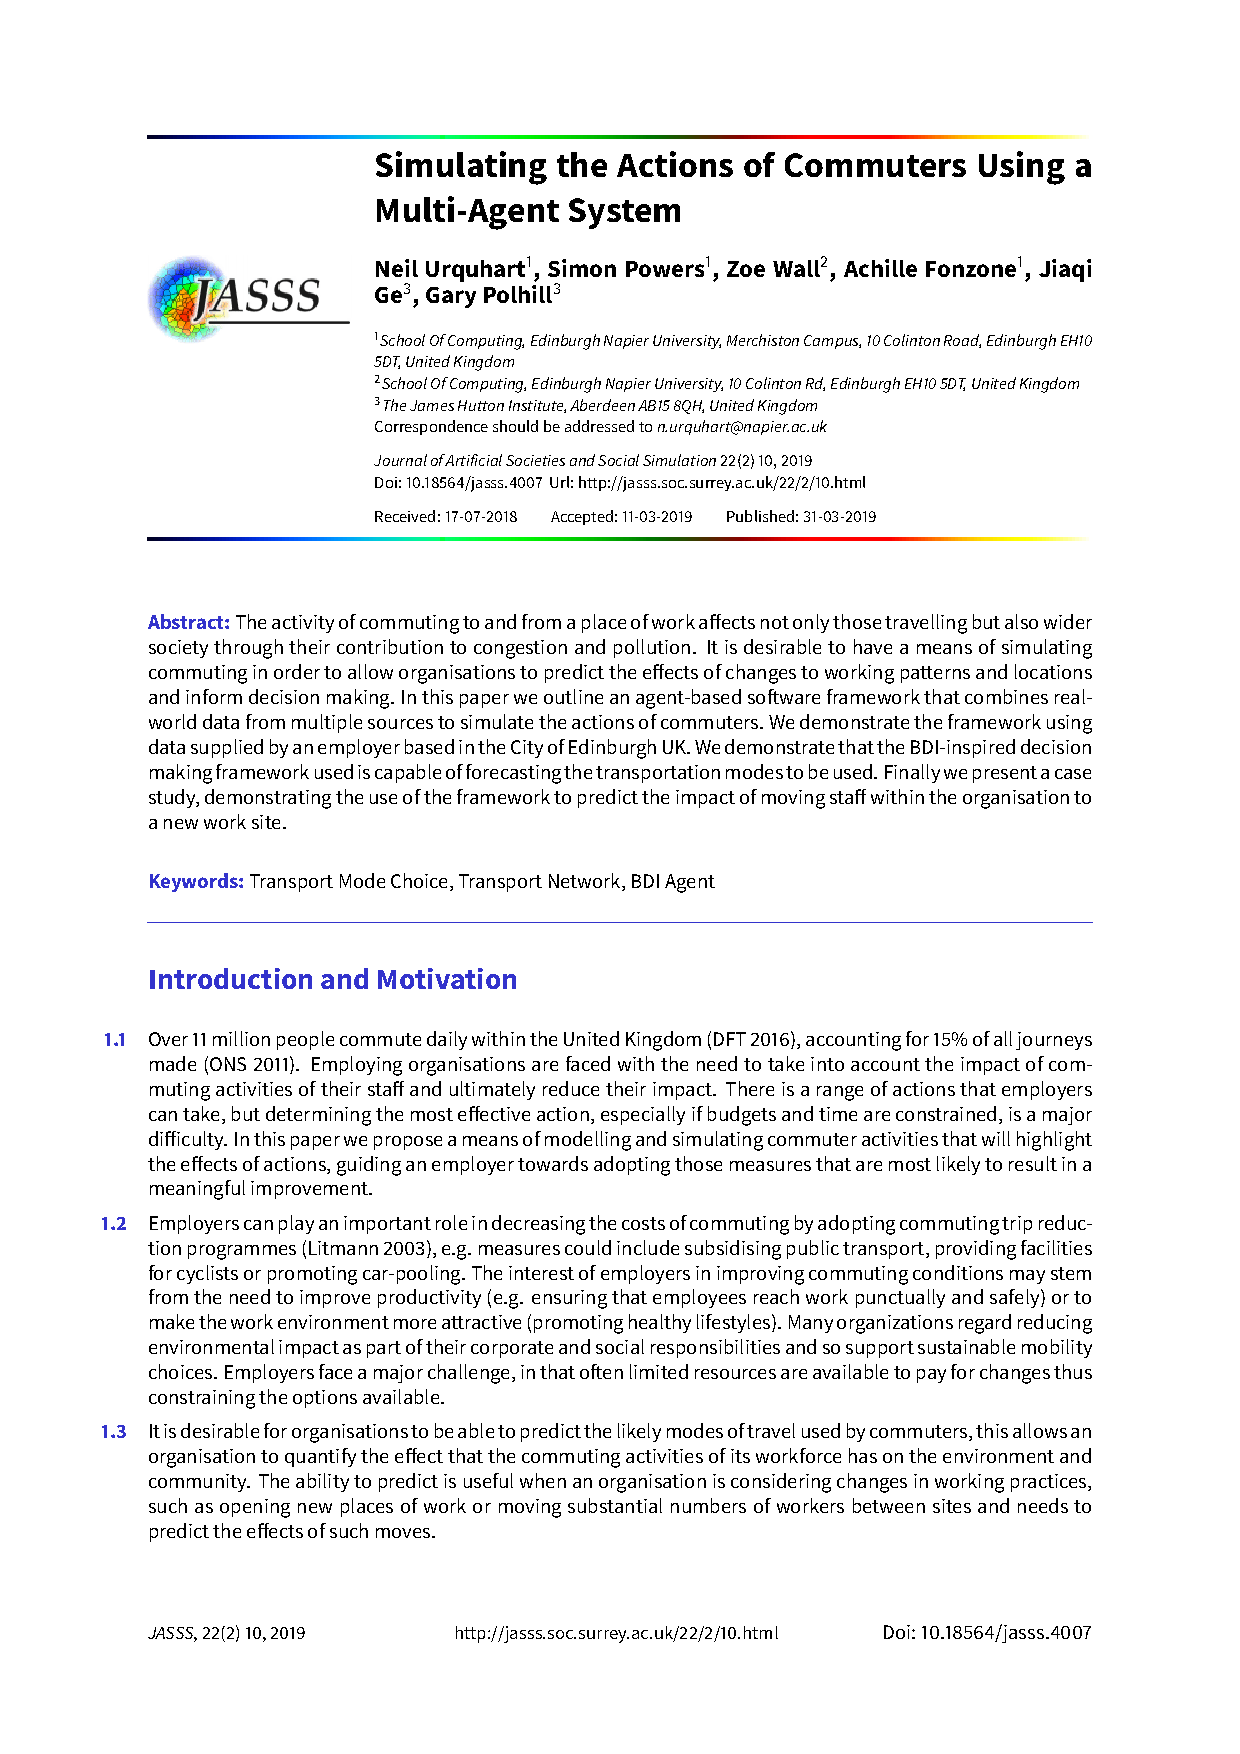
\includepdf[pages=-]{pdfs/10.18564_jasss.4007.pdf}

\chapter{Crossing the chasm: a 'tube-map' for agent-based social simulation of policy scenarios in spatially-distributed systems}

\noindent\textbf{Citation:} J G Polhill; J Ge; M P Hare; K B Matthews; A Gimona; D Salt; J Yeluripati. (2019) Crossing the chasm: a 'tube-map' for agent-based social simulation of policy scenarios in spatially-distributed systems. \textit{Geoinformatica}, 23(2), 169-199. https://doi.org/10.1007/s10707-018-00340-z

\noindent\textbf{Abstract}\par
\begin{quote}\small
Agent-based models (ABMs) simulate actions and interactions of autonomous agents and groups and their effect on systems as a whole, accounting for learning without assuming perfect rationality or complete knowledge. As such, they are well-suited to the study of complex adaptive socio-environmental systems, in which there is a need to explore the consequences of policy decisions in a context where the people whose behaviour is affected by those decisions are also able to respond and adapt to them. There has been a move away from abstract, theory-driven ABMs towards more empirically-grounded applications that stakeholders find more credible and relevant, though this introduces further challenges around validation and system description. Using Geoffrey Moore's Crossing the Chasm as a lens, we argue that the way ahead for ABM lies in identifying the niches in which it can best demonstrate its advantages, working with collaborators to show that it can deliver on its promises. We conclude by highlighting several areas requiring further development to establish ABM as an expected methodology for exploring complex socio-environmental policy scenarios in spatially-distributed systems.
\end{quote}

\vspace{0.5em}
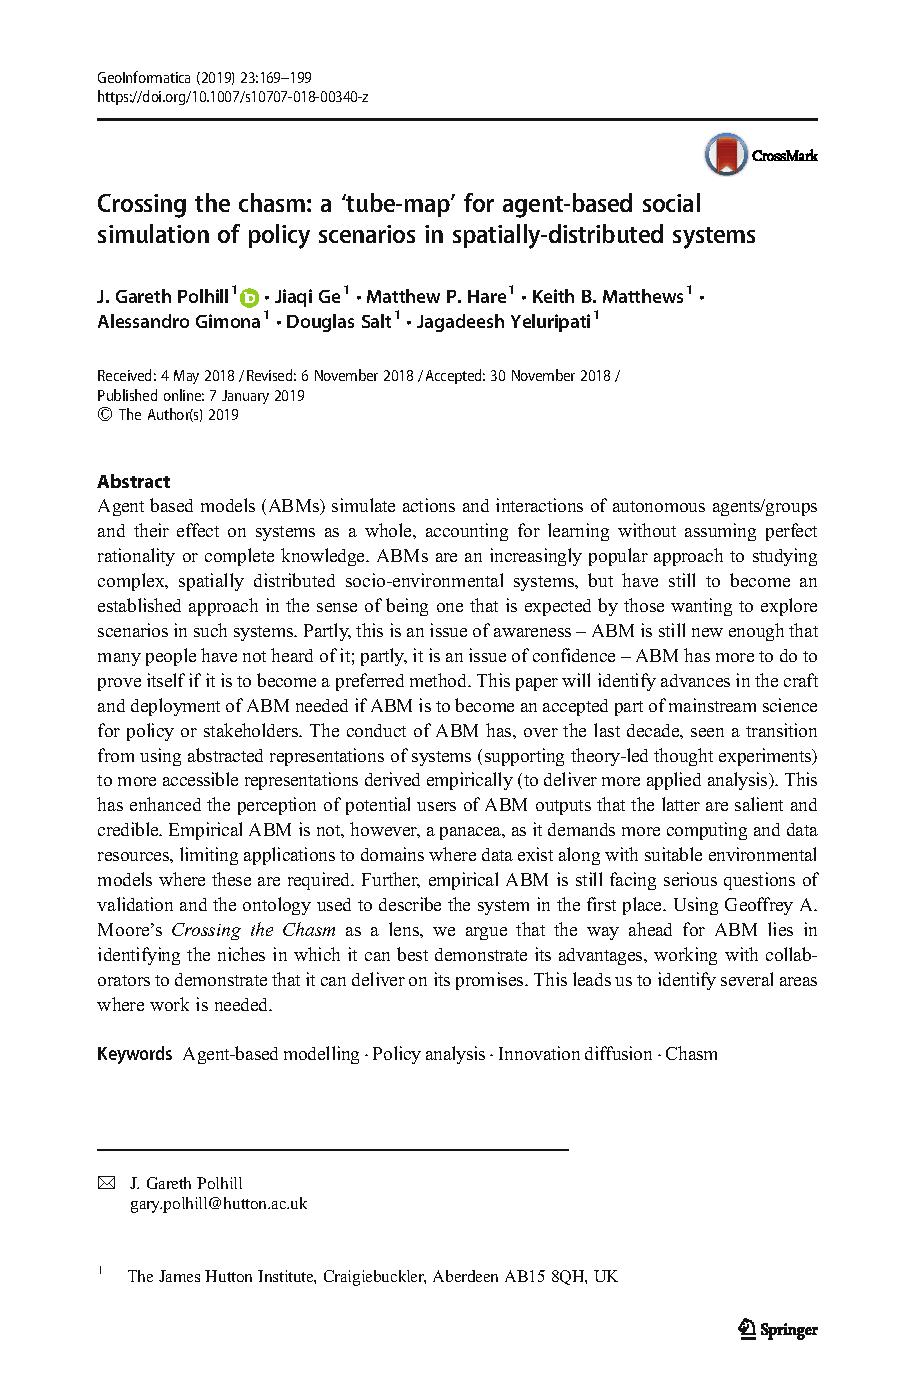
\includepdf[pages=-]{pdfs/10.1007_s10707-018-00340-z.pdf}

\chapter{Agent-based Models of Coupled Social and Natural Systems}

\noindent\textbf{Citation:} Jiaqi Ge; Gary Polhill. (2020) Agent-based Models of Coupled Social and Natural Systems. \textit{Modelling Nature-based Solutions}, 56-81. https://doi.org/10.1017/9781108553827.003

\noindent\textbf{Abstract}\par
\begin{quote}\small
Agent-based models are dynamic computer simulations that explicitly represent the interactions of heterogeneous individuals. Interest in such models stems from a number of disciplines. Some economists see agent-based models as enabling them to escape the restrictive assumptions of human rationality needed for tractable mathematical analysis under the classical paradigm, among other reasons (Axtell, 2000). Indeed, the broad affiliation of disciplines interested in a ‘complex systems’ perspective, in which systems of multiple interacting heterogeneous elements generate ‘emergent’ structure and order at the aggregate scale, offers a new metaphor for understanding economic systems. Arthur, Durlauf and Lane’s (1997) introduction to The Economy as a Complex Evolving System, for example, cites various features of real economic systems that are challenging to classical analysis, but entirely natural from a complex systems perspective: e.g. out-of-equilibrium dynamics, dispersed interaction and the lack of a global mediator. Agent-based models are closely aligned conceptually to a complex systems view of the world. Broader interest in agent-based modelling in the social sciences is derived from its perceived potential as a ‘third way’ between the quantitative and qualitative camps (Moss, 1999). The conceptual chasm between these two is often overemphasised, with most pragmatic social scientists willing to adopt mixed-methods approaches to case studies, but if seen as a formal environment in which to explore the dynamic outcomes of more assumptions than the human mind can reason with logically, agent-based models offer qualitative social scientists new tools to explore their findings, which can potentially be fitted to data gathered and analysed by quantitative social scientists. Geographers are interested in agent-based models because they can be used to represent space explicitly.
\end{quote}

\vspace{0.5em}
\chapter{Modelling food security: Bridging the gap between the micro and the macro scale}

\noindent\textbf{Citation:} Birgit Müller; Falk Hoffmann; Thomas Heckelei; Christoph Müller; Thomas W Hertel; J Gareth Polhill; Mark van Wijk; Thom Achterbosch; Peter Alexander; Calum Brown; David Kreuer; Frank Ewert; Jiaqi Ge; James D A Millington; Ralf Seppelt; Peter H Verburg; Heidi Webber. (2020) Modelling food security: Bridging the gap between the micro and the macro scale. \textit{Global Environmental Change}, 63, 102085. https://doi.org/10.1016/j.gloenvcha.2020.102085

\noindent\textbf{Abstract}\par
\begin{quote}\small
Achieving food and nutrition security for all in a changing and globalized world remains a critical challenge of utmost importance. The development of solutions benefits from insights derived from modelling and simulating the complex interactions of the agri-food system, which range from global to household scales and transcend disciplinary boundaries. A wide range of models based on various methodologies (from food trade equilibrium to agent-based) seek to integrate direct and indirect drivers of change in land use, environment and socio-economic conditions at different scales. However, modelling such interaction poses fundamental challenges, especially for representing non-linear dynamics and adaptive behaviours. We identify key pieces of the fragmented landscape of food security modelling, and organize achievements and gaps into different contextual domains of food security (production, trade, and consumption) at different spatial scales. Building on in-depth reflection on three core issues of food security -- volatility, technology, and transformation -- we identify methodological challenges and promising strategies for advancement. We emphasize particular requirements related to the multifaceted and multiscale nature of food security. They include the explicit representation of transient dynamics to allow for path dependency and irreversible consequences, and of household heterogeneity to incorporate inequality issues. To illustrate ways forward we provide good practice examples using meta-modelling techniques, non-equilibrium approaches and behavioural-based modelling endeavours. We argue that further integration of different model types is required to better account for both multi-level agency and cross-scale feedbacks within the food system.
\end{quote}

\vspace{0.5em}
\chapter{The ODD Protocol for Describing Agent-Based and Other Simulation Models: A Second Update to Improve Clarity, Replication, and Structural Realism}

\noindent\textbf{Citation:} Volker Grimm; Steven F Railsback; Christian E Vincenot; Uta Berger; Cara Gallagher; Donald L DeAngelis; Bruce Edmonds; Jiaqi Ge; Jarl Giske; Jürgen Groeneveld; Alice S A Johnston; Alexander Milles; Jacob Nabe-Nielsen; J Gareth Polhill; Viktoriia Radchuk; Marie-Sophie Rohwäder; Richard A Stillman; Jan C Thiele; Daniel Ayllón. (2020) The ODD Protocol for Describing Agent-Based and Other Simulation Models: A Second Update to Improve Clarity, Replication, and Structural Realism. \textit{Journal of Artificial Societies and Social Simulation}, 23(2). https://doi.org/10.18564/jasss.4259

\noindent\textbf{Abstract}\par
\begin{quote}\small
The Overview, Design concepts and Details (ODD) protocol for describing Individual- and Agent-Based Models (ABMs) is now widely accepted and used to document such models in journal articles. As a standardized document for providing a consistent, logical and readable account of the structure and dynamics of ABMs, some research groups also find it useful as a workflow for model design. Even so, there are still limitations to ODD that obstruct its more widespread adoption. Such limitations are discussed and addressed in this paper: the limited availability of guidance on how to use ODD; the length of ODD documents; limitations of ODD for highly complex models; lack of sufficient details of many ODDs to enable reimplementation without access to the model code; and the lack of provision for sections in the document structure covering model design rationale, the model's underlying narrative, and the means by which the model's fitness for purpose is evaluated. We document the steps we have taken to provide better guidance on: structuring complex ODDs and an ODD summary for inclusion in a journal article (with full details in supplementary material; Table 1); using ODD to point readers to relevant sections of the model code; update the document structure to include sections on model rationale and evaluation. We also further advocate the need for standard descriptions of simulation experiments and argue that ODD can in principle be used for any type of simulation model. Thereby ODD would provide a lingua franca for simulation modelling.
\end{quote}

\vspace{0.5em}
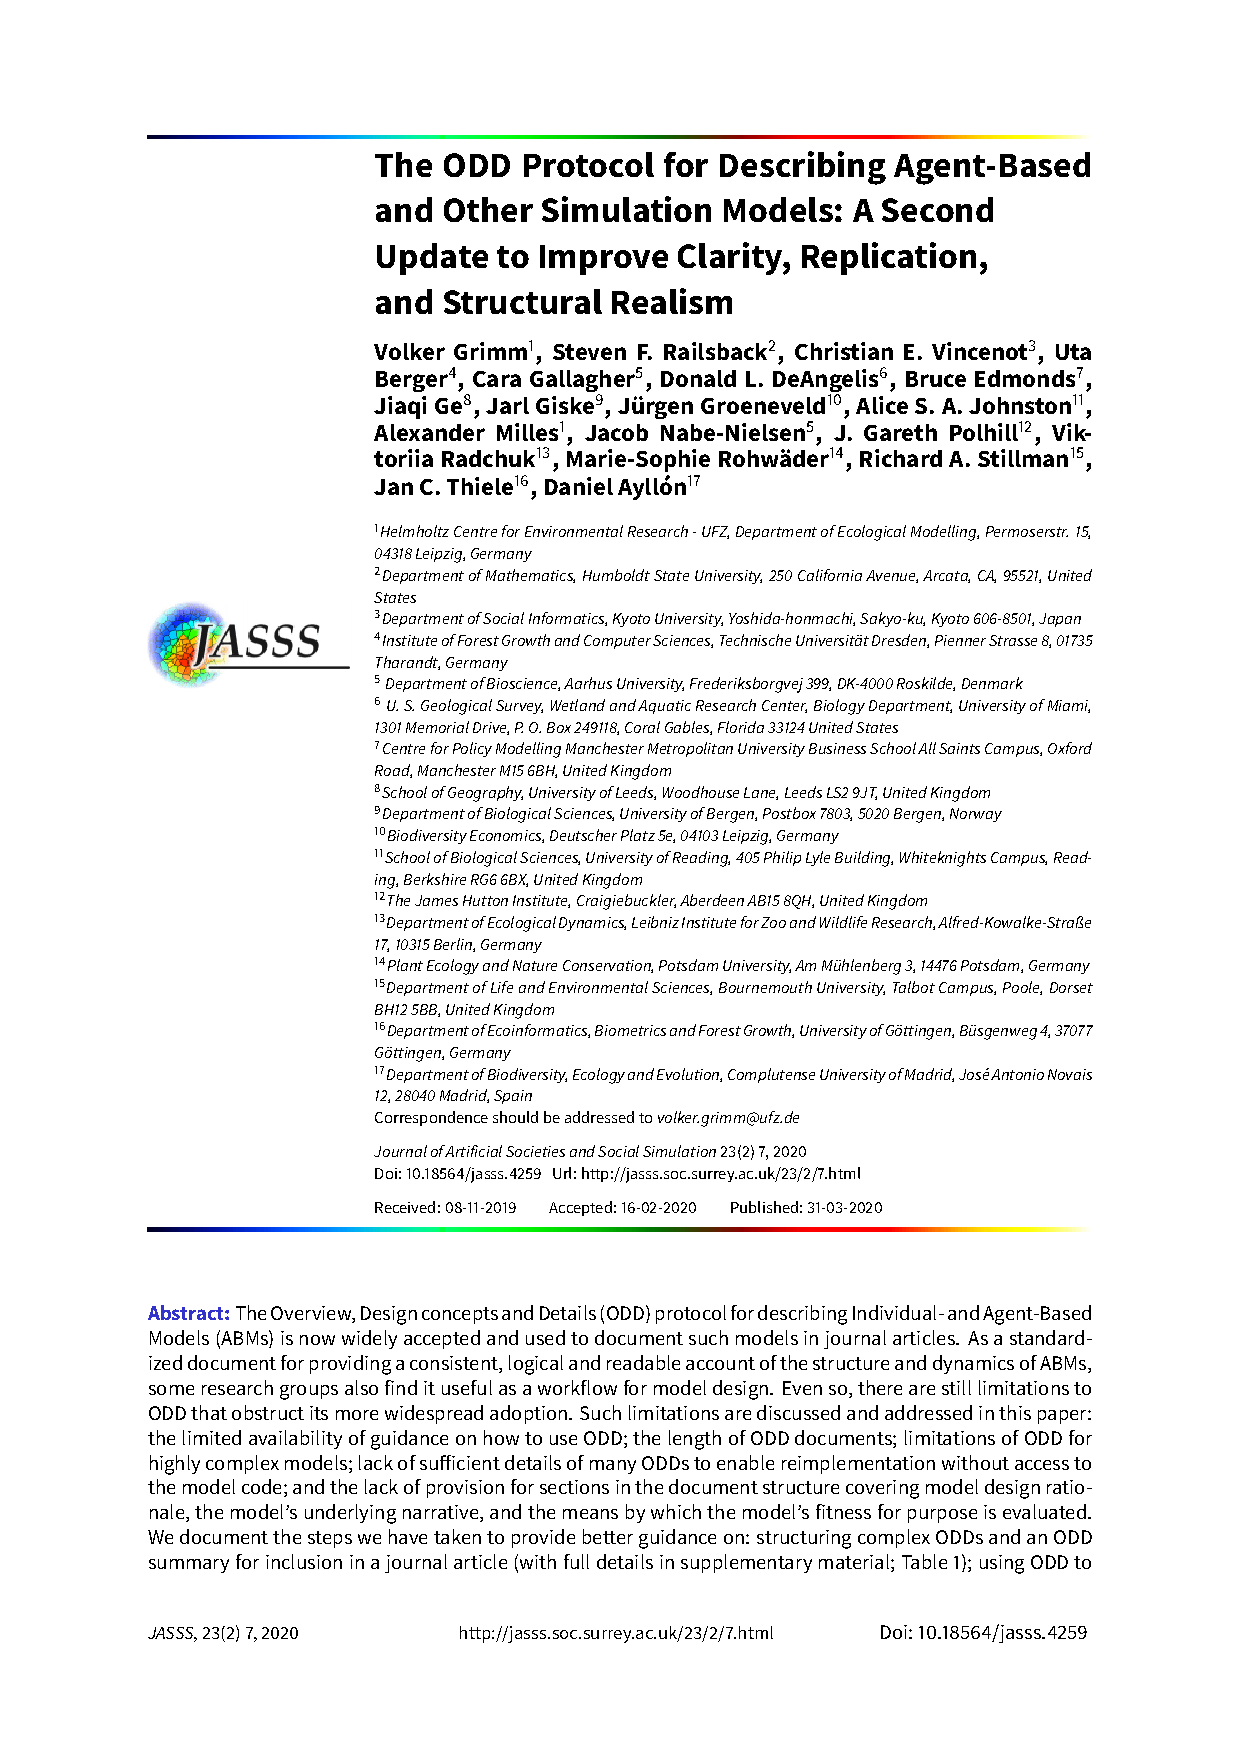
\includepdf[pages=-]{pdfs/10.18564_jasss.4259.pdf}

\chapter{Food and nutrition security under global trade: a relation-driven agent-based global trade model}

\noindent\textbf{Citation:} J Ge; J G Polhill; J I Macdiarmid; N Fitton; P Smith; H Clark; T Dawson; M Aphale. (2021) Food and nutrition security under global trade: a relation-driven agent-based global trade model. \textit{Royal Society Open Science}, 8(1), 201587. https://doi.org/10.1098/rsos.201587

\noindent\textbf{Abstract}\par
\begin{quote}\small
This paper addresses the highly relevant and timely issues of global trade and food security by developing an empirically grounded, relation-driven agent-based global trade model. Contrary to most price-driven trade models in the literature, the relation-driven agent-based global trade model focuses on the role of relational factors such as trust, familiarity, trade history and conflicts in countries' trade behaviour. Moreover, the global trade model is linked to a comprehensive nutrition formula to investigate the impact of trade on food and nutrition security, including macro and micronutrients. Preliminary results show that global trade improves the food and nutrition security of countries in Africa, Asia and Latin America. Trade also promotes a healthier and more balanced diet, as countries have access to an increased variety of food. The effect of trade in enhancing nutrition security, with an adequate supply of macro and micronutrients, is universal across nutrients and countries. As researchers call for a holistic and multifactorial approach to food security and climate change (Hammond and Dubé 2012 Proc. Natl Acad. Sci. USA 109 , 12 356–12 363. ( doi:10.1073/pnas.0913003109 )), the paper is one of the first to develop an integrated framework that consists of socio-economic, geopolitical, nutrition, environmental and agri-food systems to tackle these global challenges. Given the ongoing events of Brexit, the US–China trade war and the global COVID-19 pandemic, the paper will provide valuable insights on the role of trade in improving the food and nutrition security across countries.
\end{quote}

\vspace{0.5em}
\chapter{Future Developments in Geographical Agent‐Based Models: Challenges and Opportunities}

\noindent\textbf{Citation:} A Heppenstall; A Crooks; N Malleson; E Manley; J Ge; M Batty. (2021) Future Developments in Geographical Agent‐Based Models: Challenges and Opportunities. \textit{Geographical Analysis}, 53(1), 76-91. https://doi.org/10.1111/gean.12267

\noindent\textbf{Abstract}\par
\begin{quote}\small
Despite reaching a point of acceptance as a research tool across the geographical and social sciences, there remain significant methodological challenges for agent‐based models. These include recognizing and simulating emergent phenomena, agent representation, construction of behavioral rules, and calibration and validation. While advances in individual‐level data and computing power have opened up new research avenues, they have also brought with them a new set of challenges. This article reviews some of the challenges that the field has faced, the opportunities available to advance the state‐of‐the‐art, and the outlook for the field over the next decade. We argue that although agent‐based models continue to have enormous promise as a means of developing dynamic spatial simulations, the field needs to fully embrace the potential offered by approaches from machine learning to allow us to fully broaden and deepen our understanding of geographical systems.
\end{quote}

\vspace{0.5em}
\chapter{Simulation model of pedestrian flow based on multi-agent system and Bayesian Nash equilibrium}

\noindent\textbf{Citation:} Y Wang; J Ge; A Comber. (2021) Simulation model of pedestrian flow based on multi-agent system and Bayesian Nash equilibrium. \textit{AGILE: GIScience Series}, 2, 1-7. https://doi.org/10.5194/agile-giss-2-42-2021

\noindent\textbf{Abstract}\par
\begin{quote}\small
Abstract. Computer-based simulation is a means of exploring complex systems and has become the mainstream method of pedestrian research. In this research, a multi-agent simulation model of pedestrian flow will be established using a multi-agent system (MAS) and Bayesian Nash equilibrium. MAS is used to simulate the crowd movement and the interaction between pedestrians, and Bayesian Nash equilibrium is adopted to analyze the decision-making process of pedestrians. In contrast to previous pedestrian flow simulation modeling methods, this study adopts multi-agent modeling to realize the complete heterogeneity of pedestrians, so as to achieve more accurate simulation and make the research conclusions closer to reality. To be specific, we attempt to determine the cell side length and simulation time step of an initial model parameterized using a dataset of actual pedestrian movements. It allows more than one pedestrian to be in the same cell and stipulates that the utility of pedestrians decreases with the growing number of pedestrians in the cell. The Bayesian Nash equilibrium is applied to analyze the decision-making process of pedestrians and collision avoidance rules and interaction rules of agents are also formulated. A number of areas of further research are discussed.
\end{quote}

\vspace{0.5em}
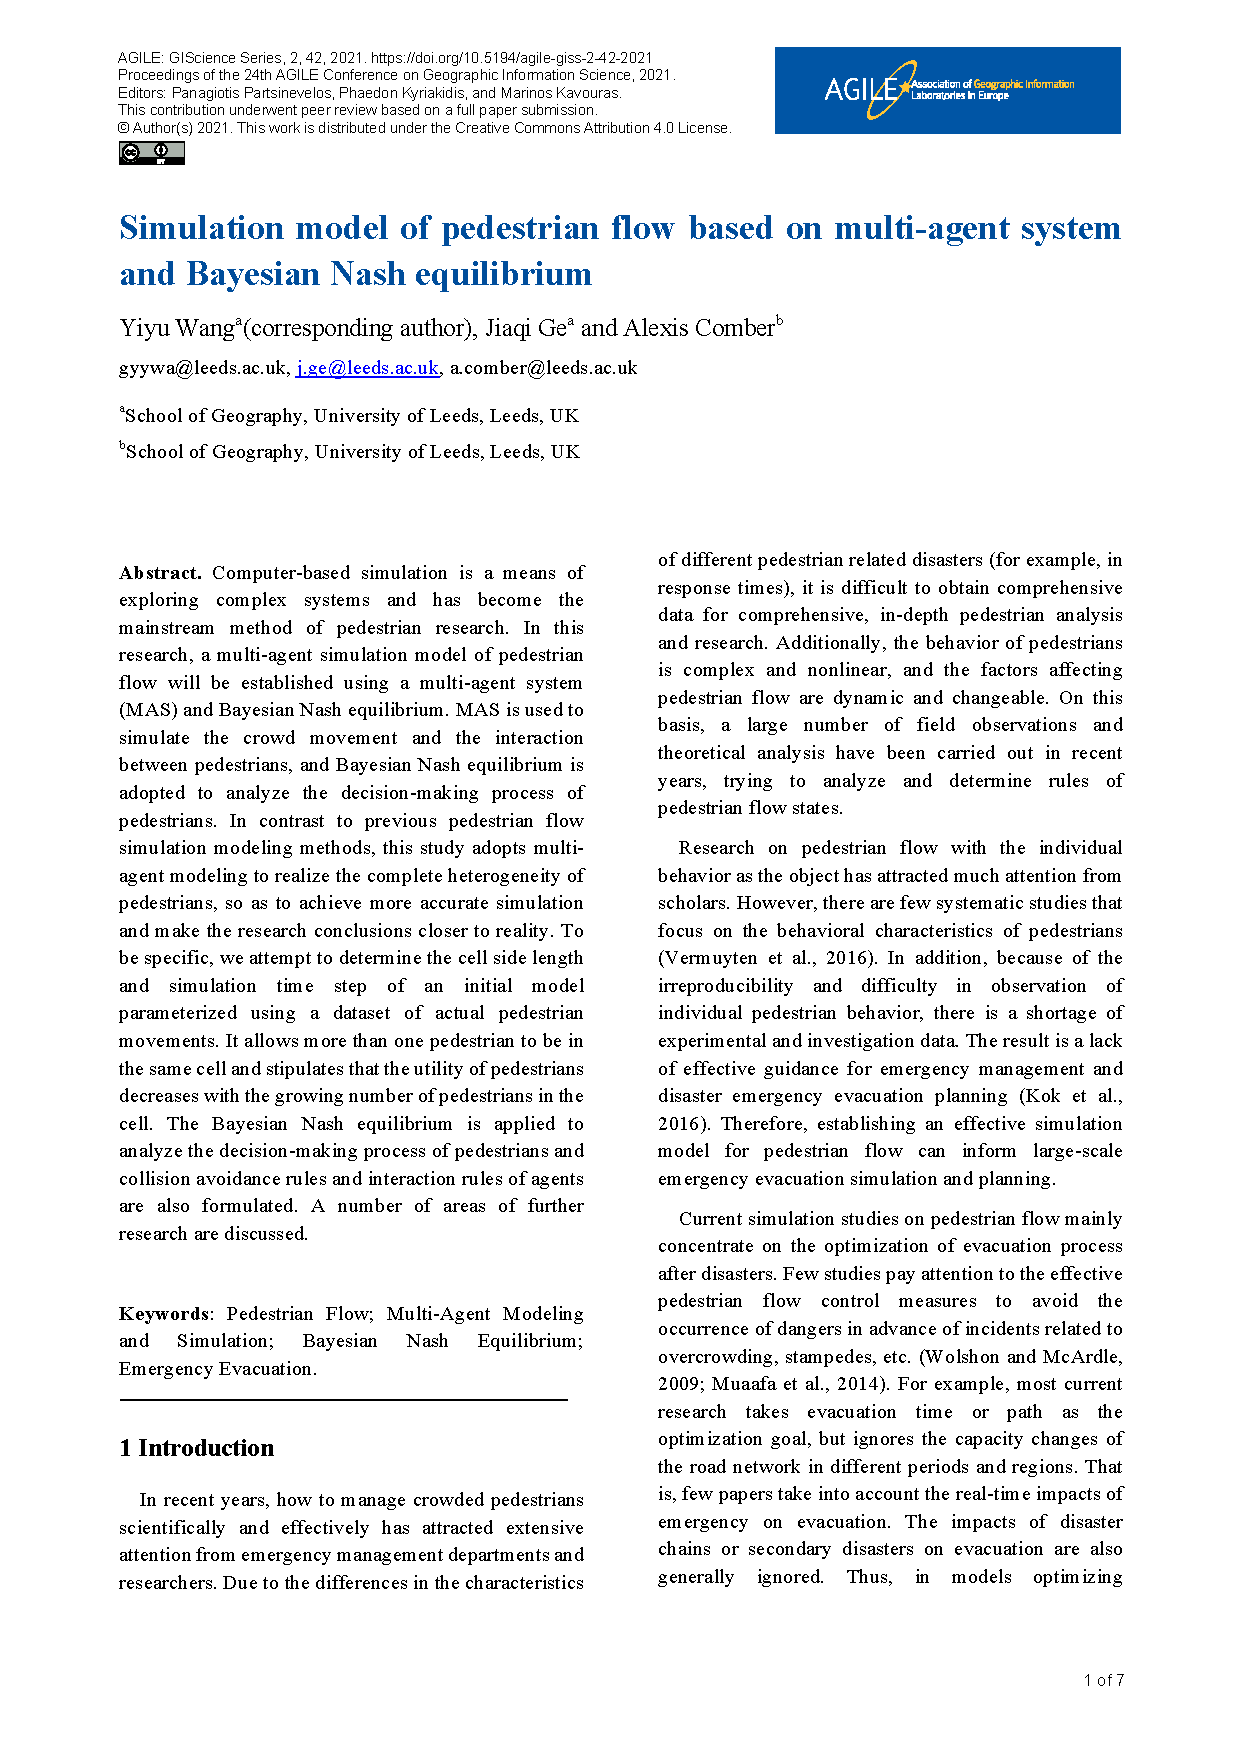
\includepdf[pages=-]{pdfs/10.5194_agile-giss-2-42-2021.pdf}

\chapter{Simulating Urban Transition in Major Socio-Economic Shocks}

\noindent\textbf{Citation:} Jiaqi Ge; Bernardo Alves Furtado. (2021) Simulating Urban Transition in Major Socio-Economic Shocks. \textit{Proceedings - Winter Simulation Conference}, 1-10. https://doi.org/10.1109/wsc52266.2021.9715510

\noindent\textbf{Abstract}\par
\begin{quote}\small
This paper presents an agent-based model that simulates the dynamic process of urban transition in major socio-economic shocks. The model examines coupled housing and labour markets across diverse neighbourhoods in a city undergoing industrial restructuring, where traditional industries are replaced by new ones. The research makes three key contributions: first, it establishes connections between housing and labour markets by linking individual and business choices to neighbourhood evolution; second, it links local workers and businesses to broader industrial structure changes within the urban system; and third, it proposes a complex systems framework for analyzing major socio-economic transitions in urban environments. Preliminary scenario analysis results from the simulation are presented.
\end{quote}

\vspace{0.5em}
\chapter{D6.1 Analysis of needs and capacity of different audiences including policy makers, expert practitioners and other modellers}

\noindent\textbf{Citation:} Milica Trajković; Dajana Vujaklija; Guy Ziv; Arjan Gosal; Jiaqi Ge; Jodi Gunning; Birgit Mueller; Annabelle Williams; Elisabet Nadeu. (2022) D6.1 Analysis of needs and capacity of different audiences including policy makers, expert practitioners and other modellers. https://doi.org/10.3897/arphapreprints.e82715

\noindent\textbf{Abstract}\par
\begin{quote}\small
This document has five main sections: the first one, \&ldquo;Developing the needs assessment protocol\&rdquo; which explains how we approached to different stakeholders in order to define and analyse their needs and capacities; the second section contains the report of of the interviews conducted by RISE and present the needs of Policy Makers; section three explains the needs of expert practitioners identified during the online workshop (14th and 15th of July 2020);\&nbsp; section four presents the needs of biophysical modeling community and section five explains the needs of ABM modellers identified from recent scholarly workshops. The results of this analysis will be taken under consideration and co-design and co-development processes.
\end{quote}

\vspace{0.5em}
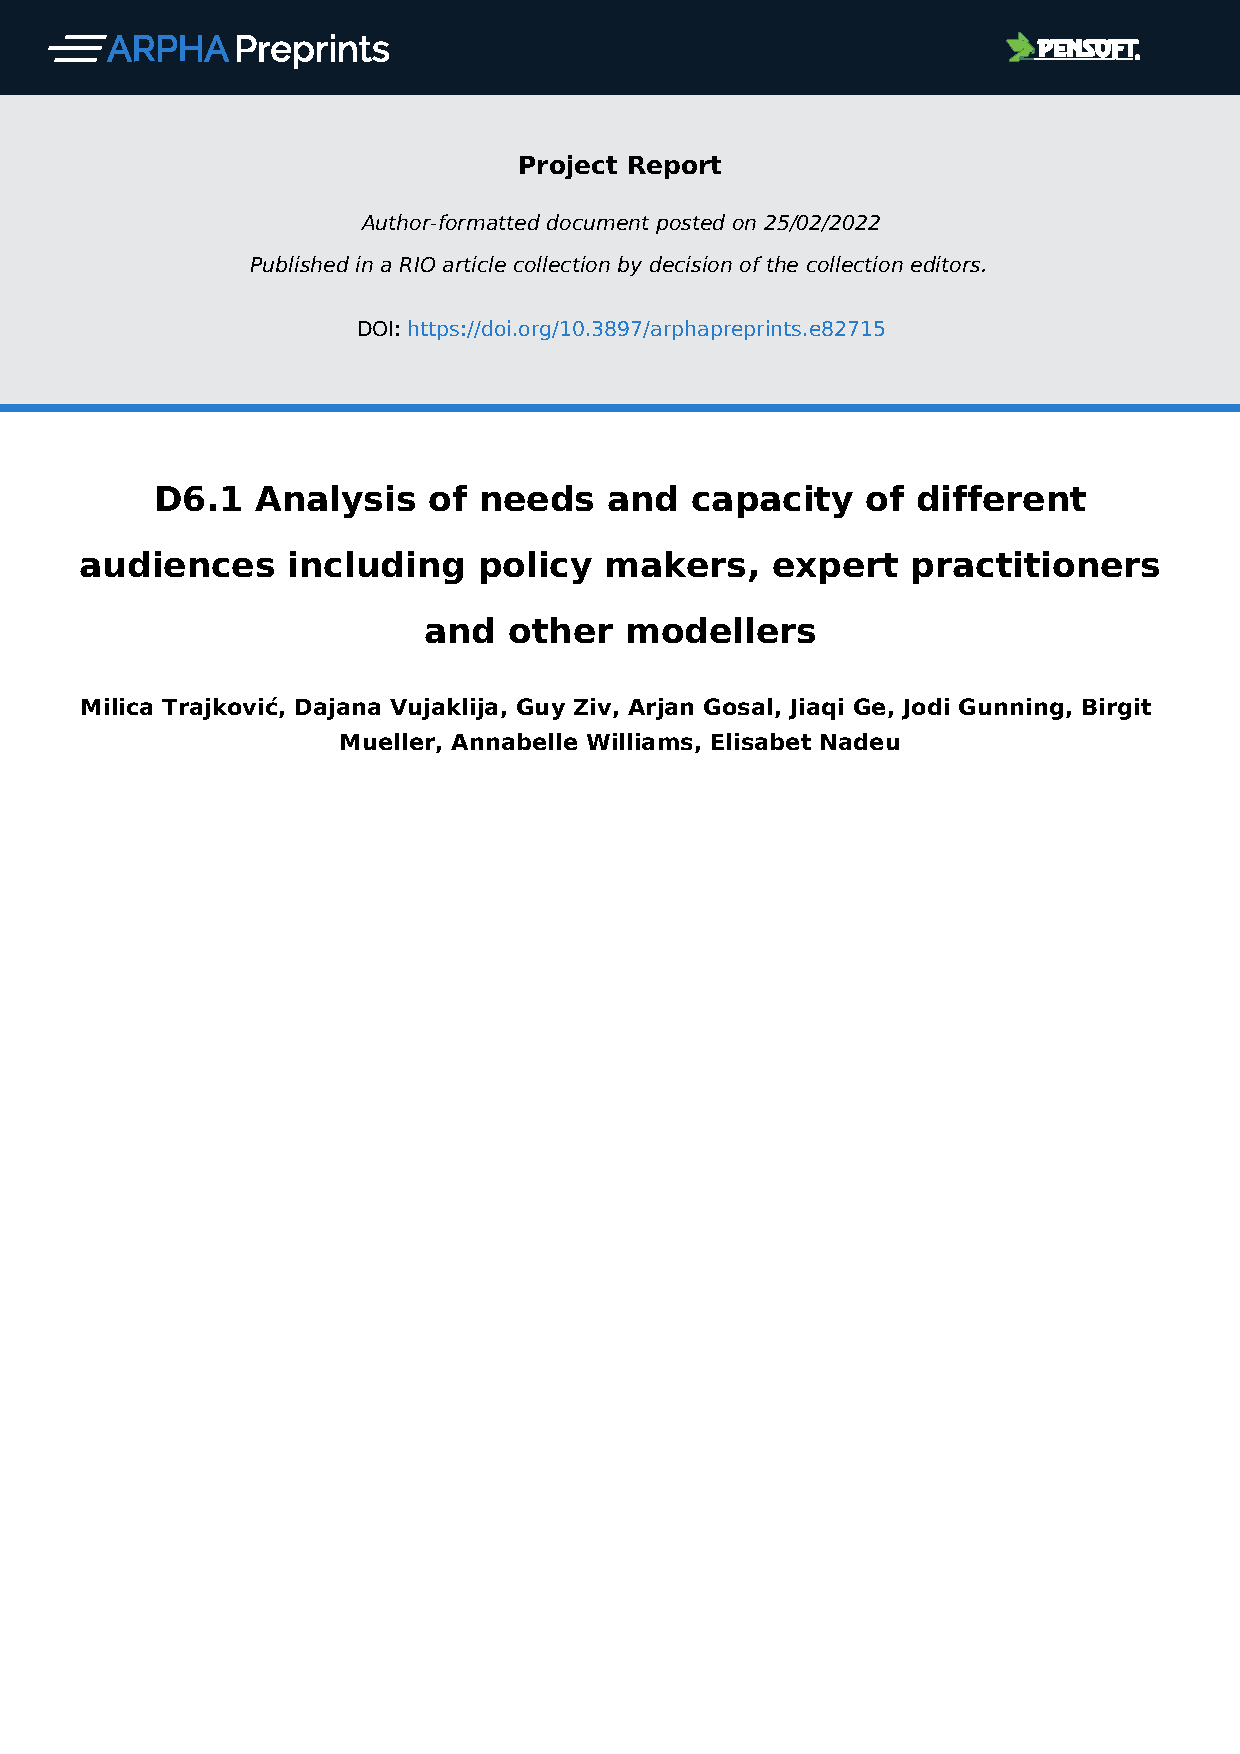
\includepdf[pages=-]{pdfs/10.3897_arphapreprints.e82715.pdf}

\chapter{Calibrating Agent-Based Models Using Uncertainty Quantification Methods}

\noindent\textbf{Citation:} J McCulloch; J Ge; J A Ward; A Heppenstall; J G Polhill; N Malleson. (2022) Calibrating Agent-Based Models Using Uncertainty Quantification Methods. \textit{Journal of Artificial Societies and Social Simulation}, 25(2). https://doi.org/10.18564/jasss.4791

\noindent\textbf{Abstract}\par
\begin{quote}\small
Agent-based models (ABMs) can be found across a number of diverse application areas ranging from simulating consumer behaviour to infectious disease modelling. Part of their popularity is due to their ability to simulate individual behaviours and decisions over space and time. However, whilst there are plentiful examples within the academic literature, these models are only beginning to make an impact within policy areas. Whilst frameworks such as NetLogo make the creation of ABMs relatively easy, a number of key methodological issues, including the quantification of uncertainty, remain. In this paper we draw on state-of-the-art approaches from the fields of uncertainty quantification and model optimisation to describe a novel framework for the calibration of ABMs using History Matching and Approximate Bayesian Computation. The utility of the framework is demonstrated on three example models of increasing complexity: (i) Sugarscape to illustrate the approach on a toy example; (ii) a model of the movement of birds to explore the efficacy of our framework and compare it to alternative calibration approaches and; (iii) the RISC model of farmer decision making to demonstrate its value in a real application. The results highlight the efficiency and accuracy with which this approach can be used to calibrate ABMs. This method can readily be applied to local or national-scale ABMs, such as those linked to the creation or tailoring of key policy decisions.
\end{quote}

\vspace{0.5em}
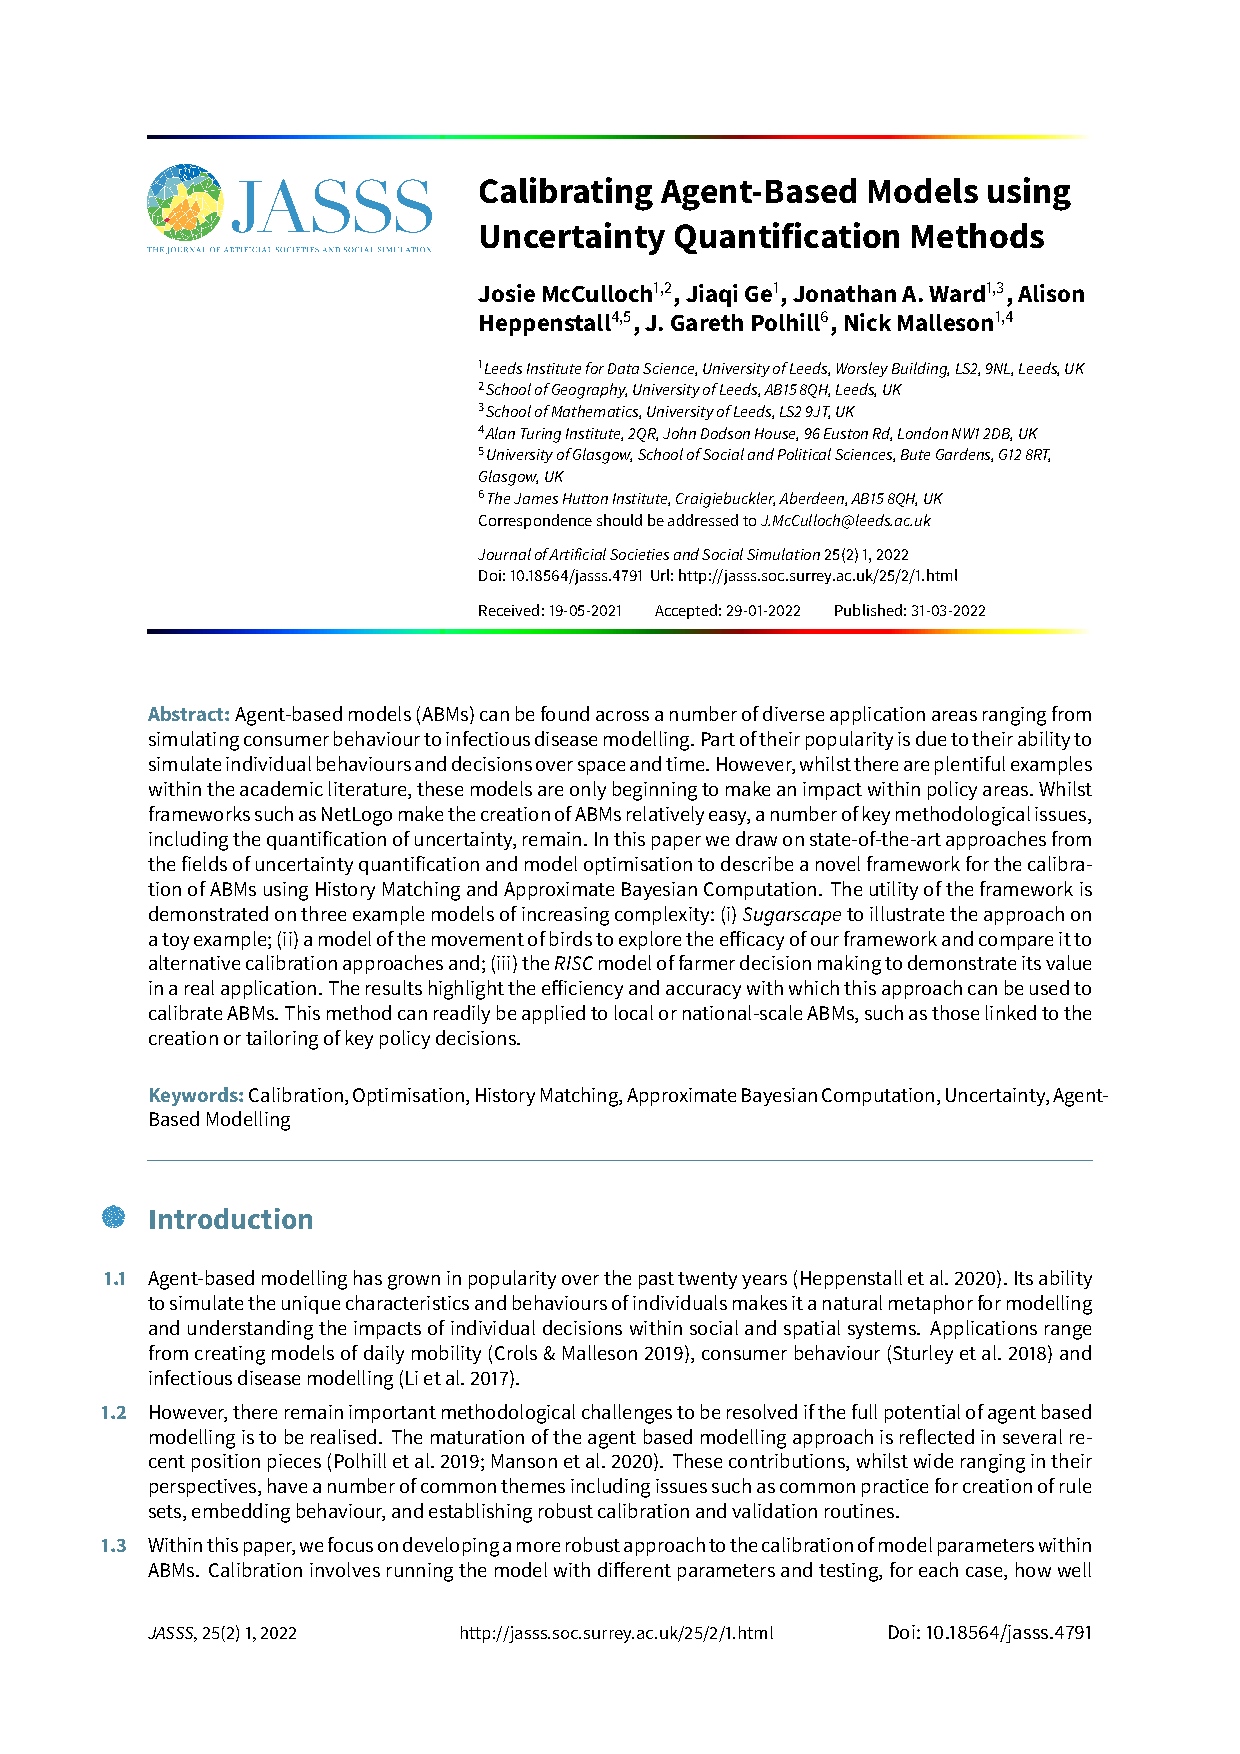
\includepdf[pages=-]{pdfs/10.18564_jasss.4791.pdf}

\chapter{Social Influence and Meat-Eating Behaviour}

\noindent\textbf{Citation:} Jiaqi Ge; Andrea Scalco; Tony Craig. (2022) Social Influence and Meat-Eating Behaviour. \textit{Sustainability}, 14(13), 7935. https://doi.org/10.3390/su14137935

\noindent\textbf{Abstract}\par
\begin{quote}\small
In recent years, interest in non-meat diets has been growing at an exponential rate in many countries. There is a wide consensus now that increased meat consumption is linked to higher health risks and environmental impact. Yet humans are social animals. Even the very personal decision of whether to eat meat or not is influenced by others around them. Using data from the British Social Attitude Survey, we develop an agent-based model to study the effect of social influence on the spread of meat-eating behaviour in the British population. We find that social influence is crucial in determining the spread of different meat-eating behaviours. According to the model, in order to bring about large-scale changes in meat-eating behaviours at the national level, people need to (1) have a strong openness to influences from others who have different meat-eating behaviour and (2) have a weak tendency to reinforce their current meat-eating behaviour after observing others in their own social group sharing the same behaviour.
\end{quote}

\vspace{0.5em}
\chapter{An evacuation simulation model of pedestrian flow using Bayesian Nash equilibrium and a Multi-Agent System}

\noindent\textbf{Citation:} Y Wang; J Ge; A Comber. (2022) An evacuation simulation model of pedestrian flow using Bayesian Nash equilibrium and a Multi-Agent System. \textit{AGILE: GIScience Series}, 3, 1-5. https://doi.org/10.5194/agile-giss-3-68-2022

\noindent\textbf{Abstract}\par
\begin{quote}\small
Abstract. The shortage of experimental data for individual behaviours has hampered systematic research on pedestrian behaviours and the refined development of evidence informed rules for pedestrian movement in simulation models. This research proposes an evacuation simulation model of pedestrian flow based on Bayesian Nash Equilibrium (BNE) and Multi-Agent System (MAS). In this paper, BNE was used to augment the logics of pedestrian decision-making processes in an evacuation MAS simulation and to improve evacuating agents’ movement and behaviours. A detailed introduction of the construction process and implementation details for the initial model as well as the visualization of experiment results are provided in this paper. Limitations and several potential future research directions are also identified.
\end{quote}

\vspace{0.5em}
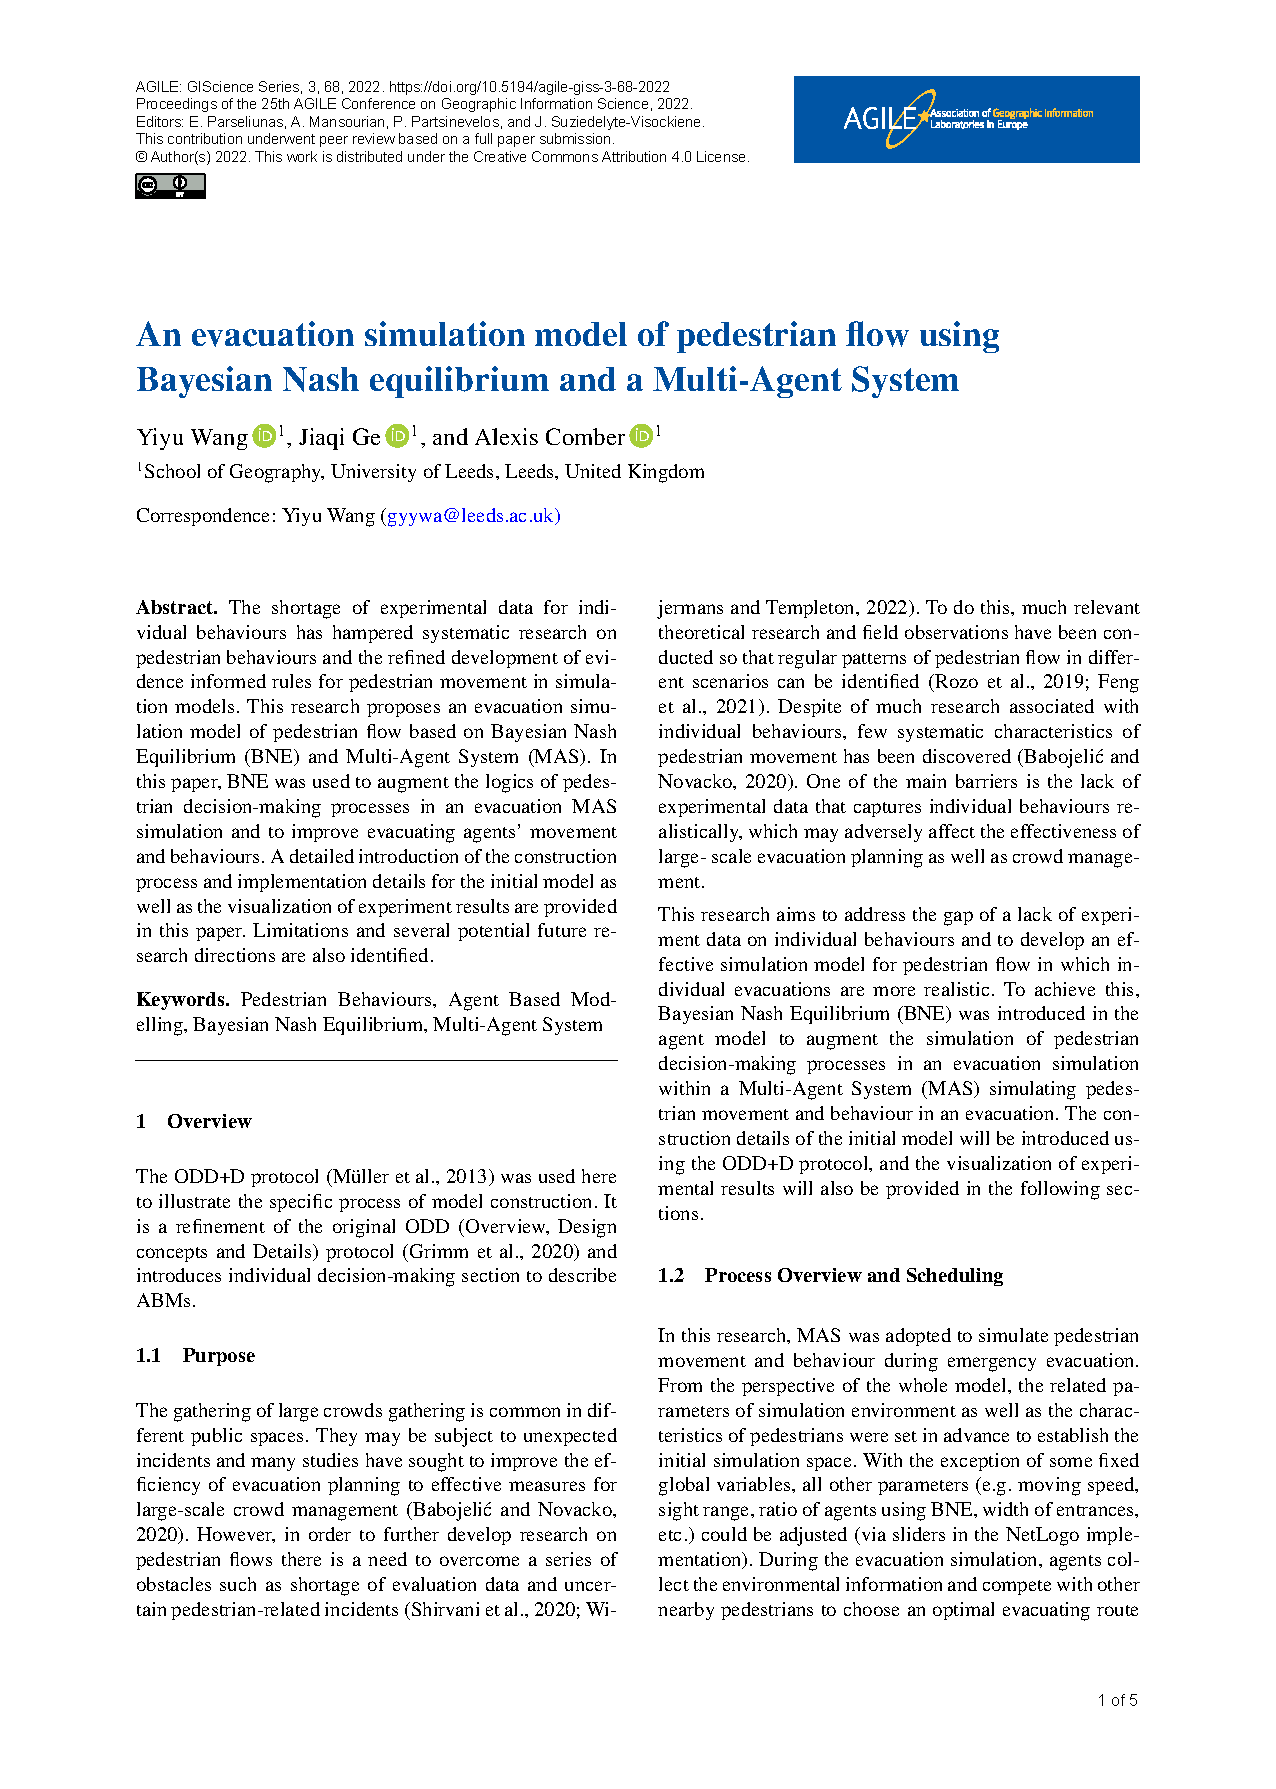
\includepdf[pages=-]{pdfs/10.5194_agile-giss-3-68-2022.pdf}

\chapter{Causal inference-informed re-analyses of factors associated with dropout from weight-loss programmes for adults}

\noindent\textbf{Citation:} R Ali; A Prestwich; J Ge; G D Tomova; C Griffiths; M S Gilthorpe. (2022) Causal inference-informed re-analyses of factors associated with dropout from weight-loss programmes for adults. \textit{Journal of Epidemiology and Community Health}, A4.1-A4. https://doi.org/10.1136/jech-2022-ssmabstracts.7

\vspace{0.5em}
\chapter{Agent-based modelling for Urban Analytics: State of the art and challenges}

\noindent\textbf{Citation:} N Malleson; M Birkin; D Birks; J Ge; A Heppenstall; E Manley; J McCulloch; P Ternes. (2022) Agent-based modelling for Urban Analytics: State of the art and challenges. \textit{AI Communications}, 35(4), 393-406. https://doi.org/10.3233/aic-220114

\noindent\textbf{Abstract}\par
\begin{quote}\small
Agent-based modelling (ABM) is a facet of wider Multi-Agent Systems (MAS) research that explores the collective behaviour of individual ‘agents’, and the implications that their behaviour and interactions have for wider systemic behaviour. The method has been shown to hold considerable value in exploring and understanding human societies, but is still largely confined to use in academia. This is particularly evident in the field of Urban Analytics; one that is characterised by the use of new forms of data in combination with computational approaches to gain insight into urban processes. In Urban Analytics, ABM is gaining popularity as a valuable method for understanding the low-level interactions that ultimately drive cities, but as yet is rarely used by stakeholders (planners, governments, etc.) to address real policy problems. This paper presents the state-of-the-art in the application of ABM at the interface of MAS and Urban Analytics by a group of ABM researchers who are affiliated with the Urban Analytics programme of the Alan Turing Institute in London (UK). It addresses issues around modelling behaviour, the use of new forms of data, the calibration of models under high uncertainty, real-time modelling, the use of AI techniques, large-scale models, and the implications for modelling policy. The discussion also contextualises current research in wider debates around Data Science, Artificial Intelligence, and MAS more broadly.
\end{quote}

\vspace{0.5em}
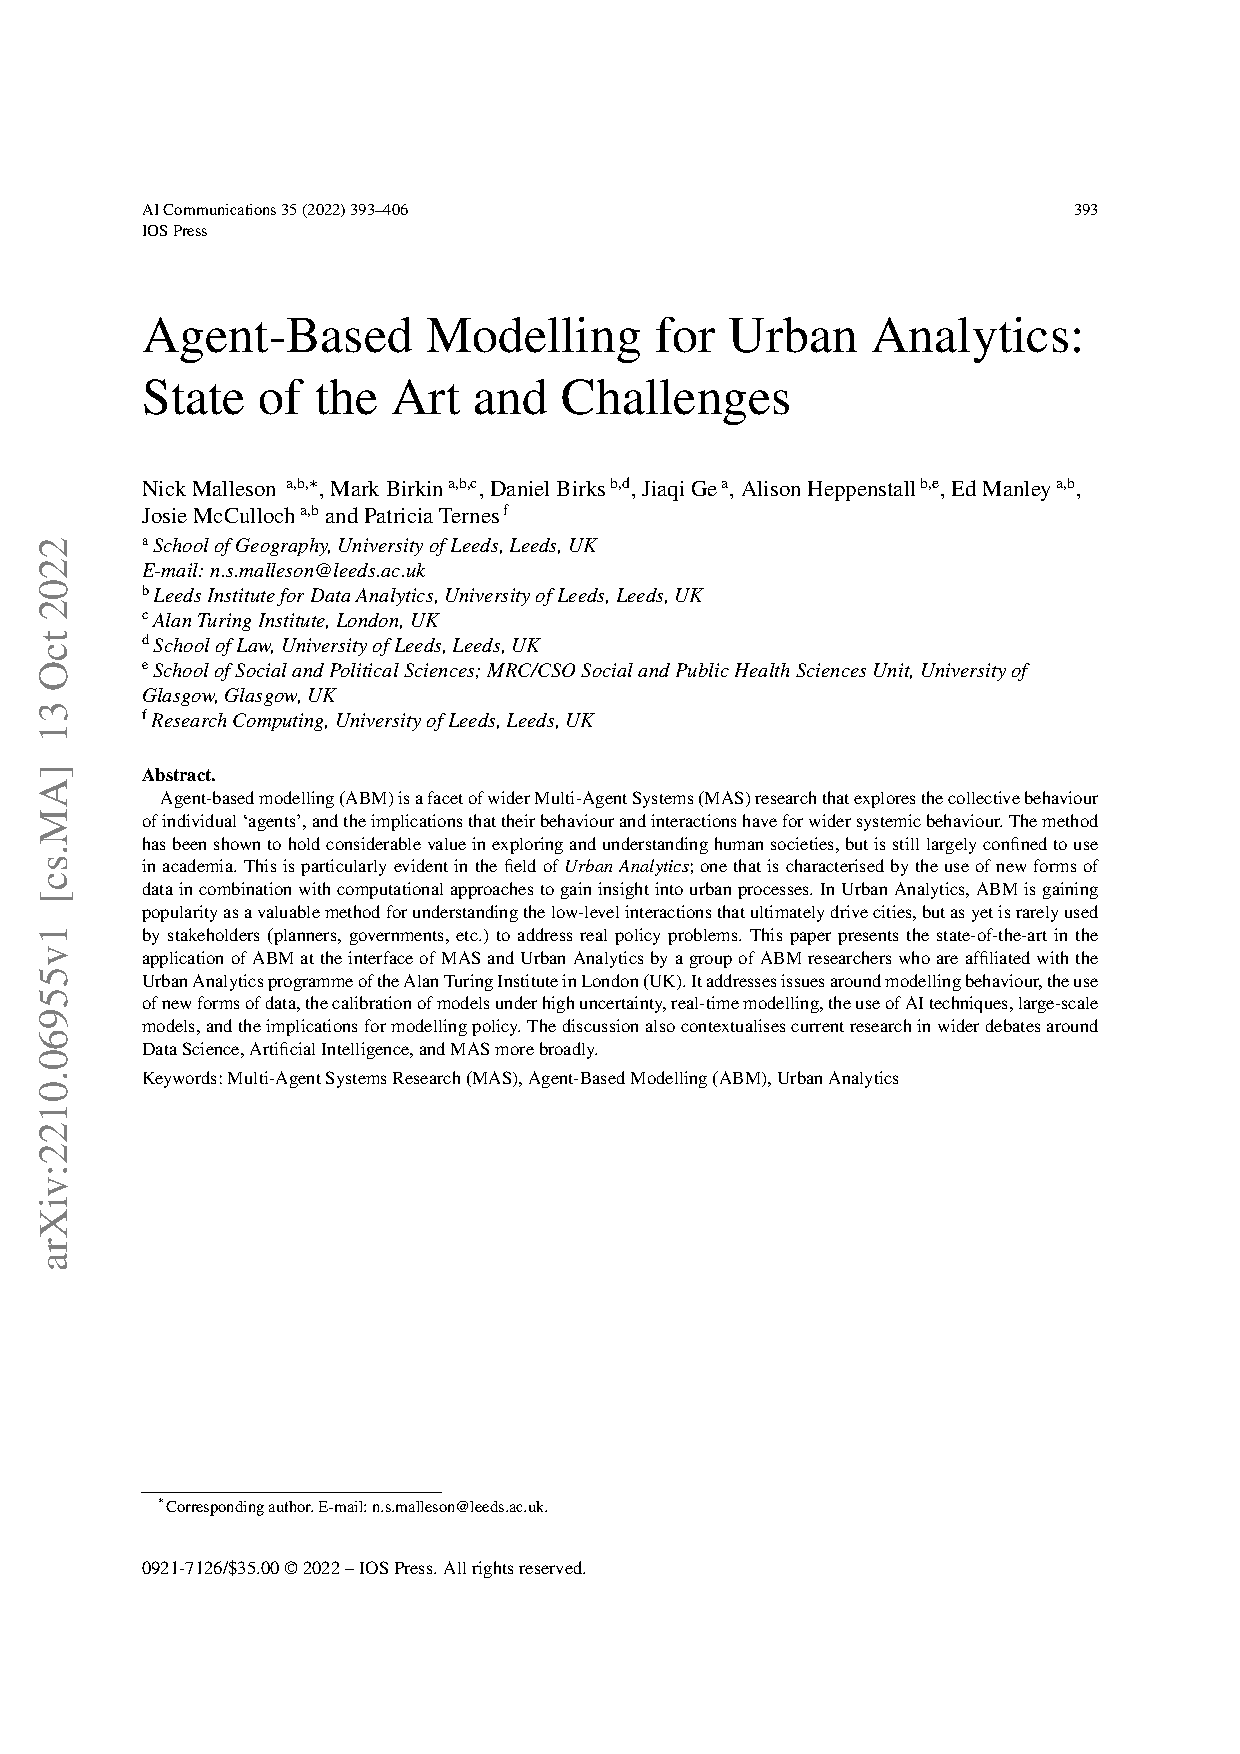
\includepdf[pages=-]{pdfs/10.3233_aic-220114.pdf}

\chapter{Introduction to the special issue on agent-based models in urban economics}

\noindent\textbf{Citation:} Jason Barr; Jiaqi Ge. (2023) Introduction to the special issue on agent-based models in urban economics. \textit{Journal of Economic Interaction and Coordination}, 18(1), 1-4. https://doi.org/10.1007/s11403-022-00375-4

\vspace{0.5em}
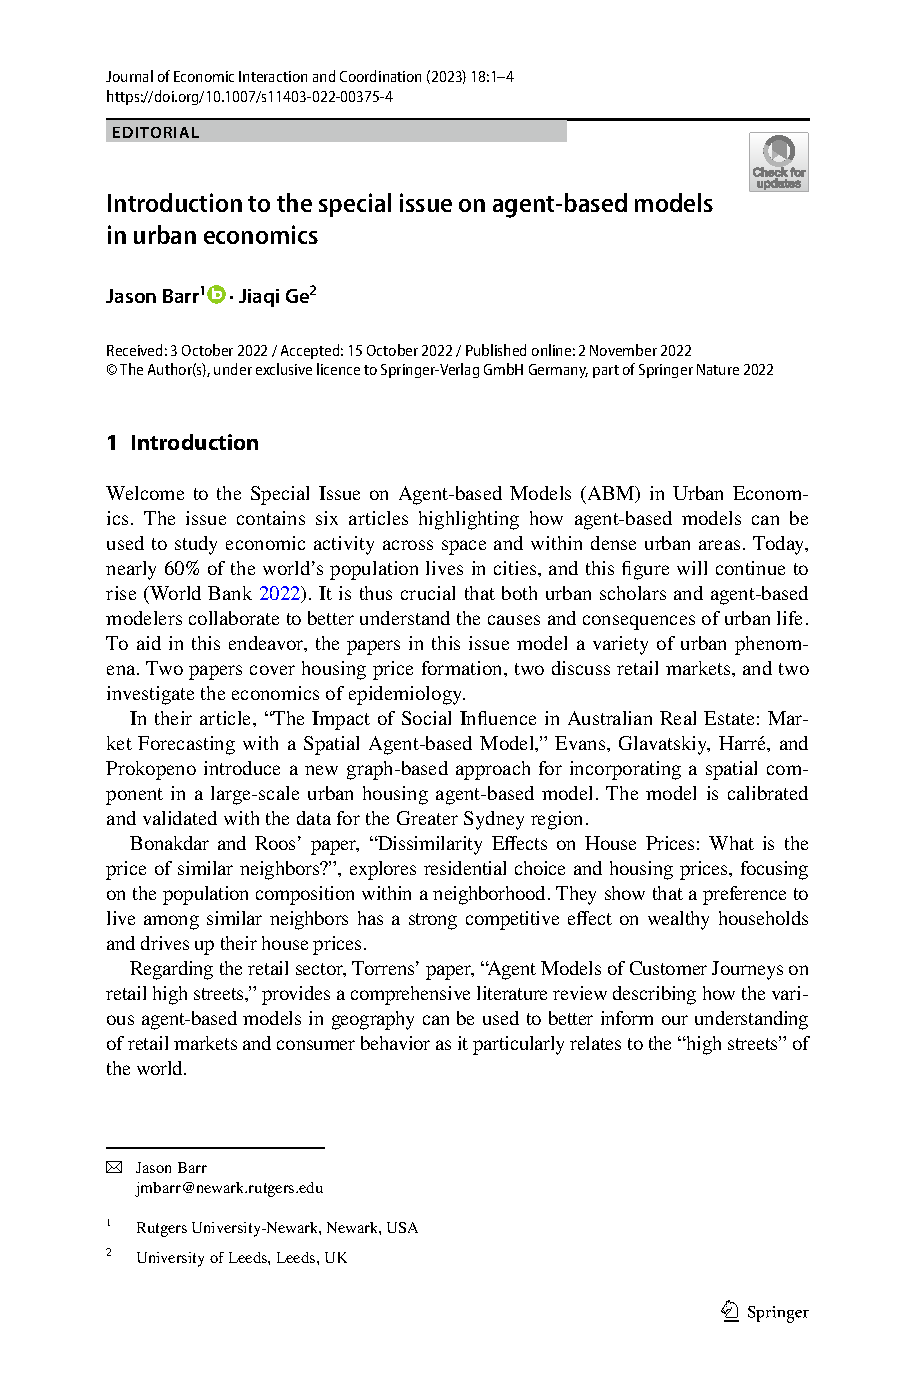
\includepdf[pages=-]{pdfs/10.1007_s11403-022-00375-4.pdf}

\chapter{An Agent-Based Simulation Model of Pedestrian Evacuation Based on Bayesian Nash Equilibrium}

\noindent\textbf{Citation:} Y Wang; J Ge; A Comber. (2023) An Agent-Based Simulation Model of Pedestrian Evacuation Based on Bayesian Nash Equilibrium. \textit{Journal of Artificial Societies and Social Simulation}, 26(3). https://doi.org/10.18564/jasss.5037

\noindent\textbf{Abstract}\par
\begin{quote}\small
This research incorporates Bayesian game theory into pedestrian evacuation in an agent-based model. Three pedestrian behaviours were compared: Random Follow, Shortest Route and Bayesian Nash Equilibrium (BNE), as well as combinations of these. The results showed that BNE pedestrians were able to evacuate more quickly as they predict congestion levels in their next step and adjust their directions to avoid congestion, closely matching the behaviours of evacuating pedestrians in reality. A series of simulation experiments were conducted to evaluate whether and how BNE affects pedestrian evacuation procedures. The results showed that: 1) BNE has a large impact on reducing evacuation time; 2) BNE pedestrians displayed more intelligent and efficient evacuating behaviours; 3) As the proportion of BNE users rises, average evacuation time decreases, and average comfort level increases. A detailed description of the model and relevant experimental results is provided in this paper. Several limitations as well as further works are also identified.
\end{quote}

\vspace{0.5em}
\includepdf[pages=-]{pdfs/10.18564_jasss.5037.pdf}

\chapter{A pedestrian ABM in complex evacuation environments based on Bayesian Nash Equilibrium}

\noindent\textbf{Citation:} Y Wang; J Ge; A Comber. (2023) A pedestrian ABM in complex evacuation environments based on Bayesian Nash Equilibrium. \textit{AGILE: GIScience Series}, 4, 1-4. https://doi.org/10.5194/agile-giss-4-50-2023

\noindent\textbf{Abstract}\par
\begin{quote}\small
Abstract. This research proposed an improved pedestrian evacuation ABM incorporating Bayesian Nash equilibrium (BNE) to provide more realistic simulations of evacuating behaviours in complex environments. BNE theory was introduced to improve the rationality of model simulations by quantifying individual decision-making process. Latest research put forward that BNE pedestrians (agents) were capable of evacuating faster and displayed more intelligent and representative evacuating behaviours. To further evaluate the role of BNE played in agents’ navigations in complex scenarios, this paper extends the above work by introducing impassable barriers with changeable sizes to realise the simulations in a more complex evacuation space with several narrow corridors. In order to match the demands of efficiently avoiding congestions and impassable areas, the decision-making rule of BNE agents when one patch was occupied by over 10 agents was improved from 100\% best strategy to a multi-strategy combination: with 50\% optimal strategy, 40\% suboptimal strategy and 10\% choosing one of the remaining options. It was found that compared with the agents following the other two traditional models, BNE agents could change their original exiting route after considering possible movements of the neighbouring agents and may evacuate through the corridors relatively further from the exit. A detailed introduction of the improved ABM is provided in this paper. Potential research directions are also identified.
\end{quote}

\vspace{0.5em}
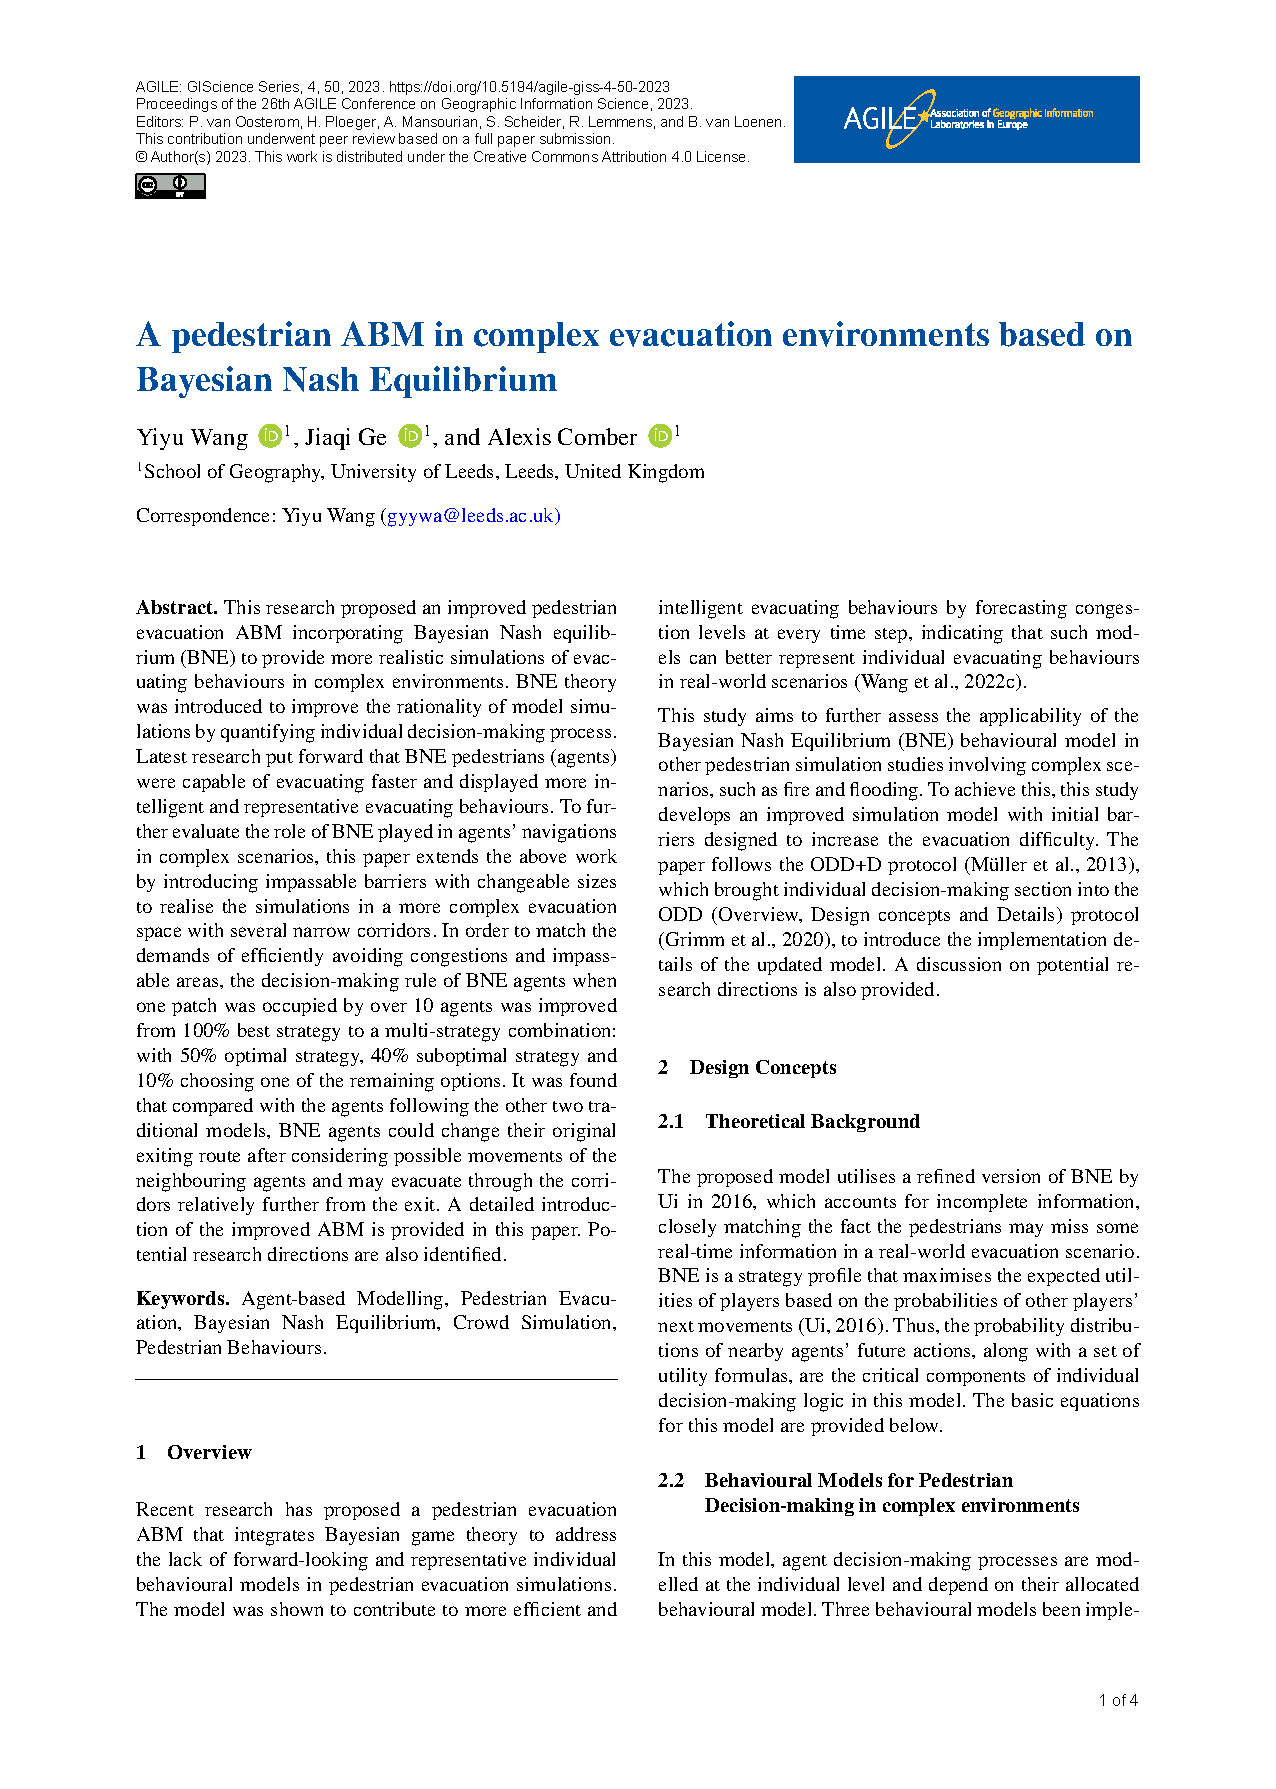
\includepdf[pages=-]{pdfs/10.5194_agile-giss-4-50-2023.pdf}

\chapter{Modelling urban transition with coupled housing and labour markets}

\noindent\textbf{Citation:} J Ge; B A Furtado. (2023) Modelling urban transition with coupled housing and labour markets. \textit{Environment and planning. B: Urban analytics and city science}, 51(3), 590-609. https://doi.org/10.1177/23998083231186623

\noindent\textbf{Abstract}\par
\begin{quote}\small
This study develops an agent-based model of urban transition, U-TRANS, with coupled housing and labour markets to simulate the transition of a city during a major industrial shift. We propose a dynamic, bottom-up framework incorporating the key interacting factors and micro mechanisms that drive the transition paths of cities. Using U-TRANS, we simulate a number of distinctive urban transition paths, from total collapse to weak recovery to enhanced training to global recruit, and analyse the resulting outcomes on economic growth, employment, inequality, housing price and the local neighbourhoods. We find that poor neighbourhoods benefit the most from growth in the new industry, whereas rich neighbourhoods do better than the rest when growth stagnates and the city declines. We also find there is a subtle trade-off between growth and equality in development strategy. By aggressively recruiting a large number of skilled workers from outside of the city in a short time, the division between local and non-local workers can be widened. The study contributes to the understanding of the dynamic process and micro mechanisms underlying urban transition. It helps explain why some cities starting from seemingly similar initial conditions may go on divergent development paths at critical moments in the history. It also demonstrates the heterogeneous impact of industrial shift on different urban neighbourhoods. The model can be used as a policy testbed for different development strategies to help cities navigate through a major industrial revolution.
\end{quote}

\vspace{0.5em}
\chapter{Navigation in Complex Space: An Bayesian Nash Equilibrium-Informed Agent-Based Model (Short Paper)}

\noindent\textbf{Citation:} Y Wang; J Ge; A Comber. (2023) Navigation in Complex Space: An Bayesian Nash Equilibrium-Informed Agent-Based Model (Short Paper). \textit{Leibniz International Proceedings in Informatics}. https://doi.org/10.4230/LIPIcs.GIScience.2023.78

\noindent\textbf{Abstract}\par
\begin{quote}\small
The lack of experimental datasets for individual behaviours has hindered the systematic studies of pedestrian behaviours as well as the refined development of regular laws of individual movement in simulation models. This research developed a simulation model for crowd evacuation on the basis of Bayesian Nash Equilibrium (BNE) and a Multi-Agent System (MAS). BNE was introduced in this research to augment the rationality of individual decision-making process in evacuation simulation and to assist pedestrians in discovering an optimal evacuation route to avoid congestions. A series of simulation experiments were conducted to evaluate the performance of the initial model, and the current experimental results demonstrate a noticeable positive influence of BNE on reducing evacuation time. A detailed introduction of the establishment and implementation details of the model as well as model analysis have been provided in this paper. Limitations and a few optional research directions in the future are also discussed.
\end{quote}

\vspace{0.5em}
\chapter{An Agent-Based Model of UK Farmers’ Decision-Making on Adoption of Agri-environment Schemes}

\noindent\textbf{Citation:} Chunhui Li; Meike Will; Nastasija Grujić; Jiaqi Ge; Birgit Müller; Arjan Gosal; Guy Ziv. (2023) An Agent-Based Model of UK Farmers’ Decision-Making on Adoption of Agri-environment Schemes. \textit{Springer Proceedings in Complexity}, 463-475. https://doi.org/10.1007/978-3-031-34920-1\_37

\noindent\textbf{Abstract}\par
\begin{quote}\small
Agri-environment schemes (AES) are government-funded voluntary programs that incentivise farmers and land managers for environmentally friendly farming practices. Understanding farmers' decision-making process and its impact on AES adoption can aid policy makers in designing AES schemes that meet adoption goals and environmental targets. This paper presents a spatially explicit agent-based model (ABM) -- BESTMAP-ABM-UK -- that simulates farmers' decision-making process, inclusive of farmers' social, behavioural and economic factors, on adopting buffer strips, cover crops, grassland management and arable land conversion to grassland schemes in the UK. The model produces farmers' AES adoption under varied AES scheme designs in terms of the contract length, the offered payment level, the bureaucracy level and the required minimal area.
\end{quote}

\vspace{0.5em}
\chapter{A Preliminary Study of Individual Based Crowd Simulation Based on Bayesian Nash Equilibrium}

\noindent\textbf{Citation:} Yiyu Wang; Jiaqi Ge; Alexis Comber. (2023) A Preliminary Study of Individual Based Crowd Simulation Based on Bayesian Nash Equilibrium. \textit{Springer Proceedings in Complexity}, 329-336. https://doi.org/10.1007/978-3-031-34920-1\_26

\noindent\textbf{Abstract}\par
\begin{quote}\small
The lack of experimental datasets for individual behaviours has hindered the systematic studies of pedestrian behaviours as well as the refined development of regular laws of individual movement in simulation models. This research developed a simulation model for crowd evacuation on the basis of Bayesian Nash Equilibrium (BNE) and a Multi-Agent System (MAS). BNE was introduced in this research to augment the rationality of individual decision-making process in evacuation simulation and to assist pedestrians in discovering an optimal evacuation route to avoid congestions. A series of simulation experiments were conducted to evaluate the performance of the initial model, and the current experimental results demonstrate a noticeable positive influence of BNE on reducing evacuation time.
\end{quote}

\vspace{0.5em}
\chapter{Mitigating housing market shocks: an agent-based reinforcement learning approach with implications for real-time decision support}

\noindent\textbf{Citation:} S Olmez; A Heppenstall; J Ge; C Elsenbroich; D Birks. (2024) Mitigating housing market shocks: an agent-based reinforcement learning approach with implications for real-time decision support. \textit{Journal of Simulation}, 18(6), 921-939. https://doi.org/10.1080/17477778.2024.2375446

\noindent\textbf{Abstract}\par
\begin{quote}\small
Research in modelling housing market dynamics using agent-based models (ABMs) has grown due to the rise of accessible individual-level data. This research involves forecasting house prices, analysing urban regeneration, and the impact of economic shocks. There is a trend towards using machine learning (ML) algorithms to enhance ABM decision-making frameworks. This study investigates exogenous shocks to the UK housing market and integrates reinforcement learning (RL) to adapt housing market dynamics in an ABM. Results show agents can learn real-time trends and make decisions to manage shocks, achieving goals like adjusting the median house price without pre-determined rules. This model is transferable to other housing markets with similar complexities. The RL agent adjusts mortgage interest rates based on market conditions. Importantly, our model shows how a central bank agent learned conservative behaviours in sensitive scenarios, aligning with a 2009 study, demonstrating emergent behavioural patterns.
\end{quote}

\vspace{0.5em}
\chapter{Learning the rational choice perspective: A reinforcement learning approach to simulating offender behaviours in criminological agent-based models}

\noindent\textbf{Citation:} S Olmez; D Birks; A Heppenstall; J Ge. (2024) Learning the rational choice perspective: A reinforcement learning approach to simulating offender behaviours in criminological agent-based models. \textit{Computers, Environment and Urban Systems}, 112, 102141. https://doi.org/10.1016/j.compenvurbsys.2024.102141

\noindent\textbf{Abstract}\par
\begin{quote}\small
Over the past 15 years, environmental criminologists have explored the application of agent-based models (ABMs) of crime events and various theoretical frameworks applied to understand them. Models have supported criminological theorising and, in some cases, been applied to make predictions about the impact of interventions devised to reduce crime. However, decision-making frameworks utilised in criminological ABMs have typically been implemented through traditional techniques such as condition-action rules. While these models have provided significant insights, they neglect a crucial component of theoretical accounts of offending, the notion that offenders are learning agents whose behavioural dynamics change over time and space. In response, this article presents an ABM of residential burglary in which offender agents utilise reinforcement learning (RL) to learn behaviours. This solution enables offender agents to learn from individual-level perceptions of the environment and, given these perceptions, develop behavioural responses that benefit themselves. The model includes conceptualisations of the Routine Activity Theory (RAT), Crime Pattern Theory (CPT) and a utility function, Target Attractiveness, which acts as a behavioural mould to nudge offender agents to learn behaviours in keeping with the Rational Choice Perspective (RCP). Trained behaviours are then tested by introducing crime prevention interventions into the model and examining the reactions of offender agents. In keeping with empirical studies of offending, experimental results demonstrate that offender agents utilising RL learn to offend at targets where rewards outweigh risks and effort, offend close to home, frequently victimise high-rewarding targets, and conversely learn to avoid offending in areas associated with high levels of risk and effort.
\end{quote}

\vspace{0.5em}
\chapter{From primary data to formalized decision-making: Open challenges and ways forward to inform representations of farmers' behaviour in agent-based models}

\noindent\textbf{Citation:} G Ziv; J Ge. (2024) From primary data to formalized decision-making: Open challenges and ways forward to inform representations of farmers' behaviour in agent-based models. \textit{Ecology and Society}, 29(4). https://doi.org/10.5751/ES-15400-290431

\noindent\textbf{Abstract}\par
\begin{quote}\small
Model-based analyses effectively investigate leverage points for sustainability transformations in agriculture by systematically evaluating policies under varying environmental, economic, or institutional conditions. Agent-based modeling proves particularly valuable for analyzing agricultural systems because it represents individual farmers -- key actors in land use -- their interactions, and resulting landscape-level patterns. However, formalizing empirically observed farmer behavior into model rules presents challenges, especially with qualitative data. This article guides modelers through formalizing farmer decision-making based on empirical findings in three steps: selecting approach, choosing key elements, and translating findings. The authors illustrate their framework using literature examples and their own model representing farmer decision-making regarding agri-environmental scheme adoption across Europe. By systematizing this process, agent-based models become less stylized, offering greater potential for supporting policymakers in identifying sustainable agricultural transformation strategies.
\end{quote}

\vspace{0.5em}
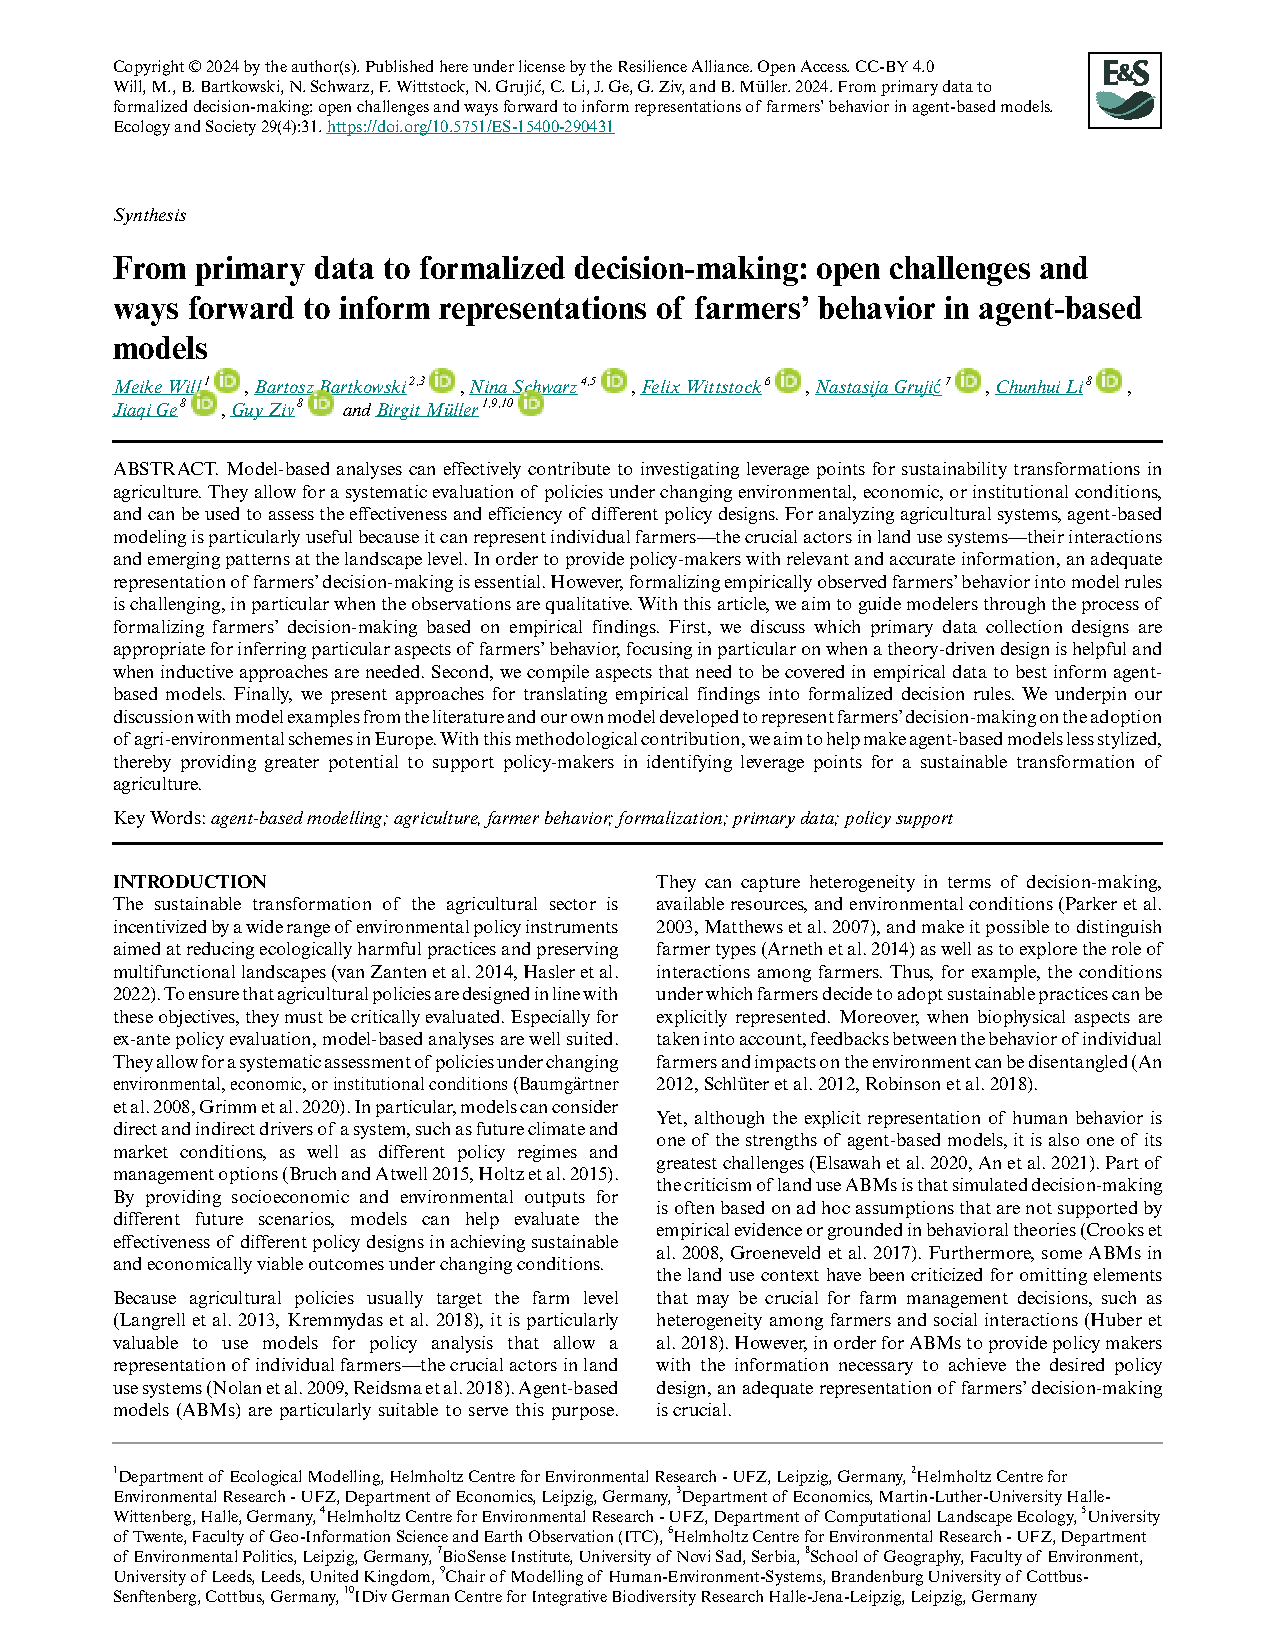
\includepdf[pages=-]{pdfs/10.5751_ES-15400-290431.pdf}

\chapter{Predicting adoption of agri-environmental schemes by farmers in the European Union}

\noindent\textbf{Citation:} J McCulloch; J Ge. (2025) Predicting adoption of agri-environmental schemes by farmers in the European Union. \textit{PLOS Sustainability and Transformation}, 4(3), e0000162. https://doi.org/10.1371/journal.pstr.0000162

\noindent\textbf{Abstract}\par
\begin{quote}\small
Much of the land across the European Union (EU) is threatened by unsustainable land-use through intensive farming. To help combat this, Agri-Environmental Schemes (AESs) are provided by the EU to encourage farmers to use a portion of their land to aid with environmental goals such as sustainable farming, bio-diversity or landscape recovery. Farmers in the EU are given the opportunity to take on an AES for a monetary payment that is based on the choice of scheme and the amount of land dedicated to it. If we know or can accurately predict which farmers adopt which AES, we can then predict if the intended benefits to the environment according to the given scheme are likely to be achieved. As a preliminary step, we develop a generalised linear model coupled with a microsimulation that is fed with data from the Farm Accountancy Data Network to predict AES uptake. We find the model is able to accurately predict approximately 70\% of farmers’ decisions on whether to adopt an AES across 27 countries in the EU. In the future, this model can be used to predict, for example, if the chosen schemes adopted will lead to their intended benefits, and if changes in the offered AES payment may affect AES adoption.
\end{quote}

\vspace{0.5em}
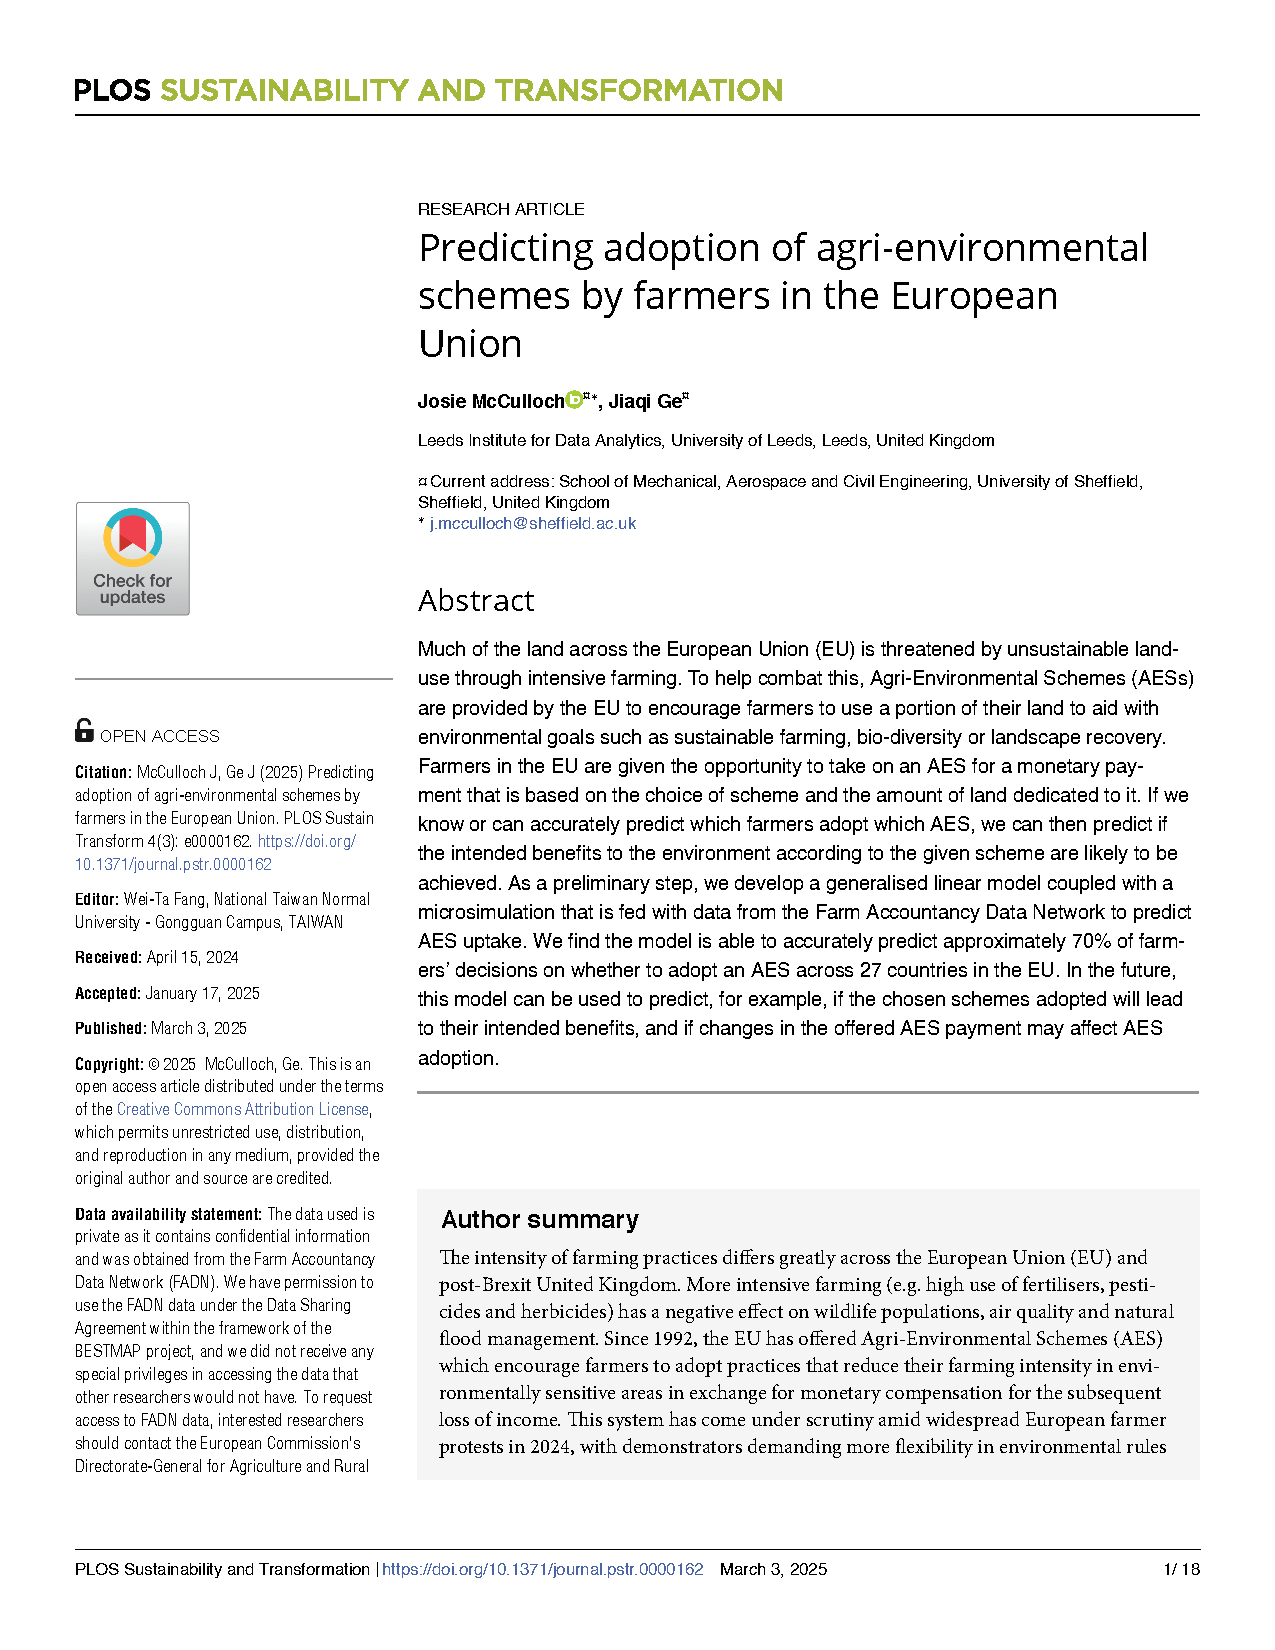
\includepdf[pages=-]{pdfs/10.1371_journal.pstr.0000162.pdf}

\chapter{Composite variable bias: causal analysis of weight outcomes}

\noindent\textbf{Citation:} R Ali; A Prestwich; J Ge; C Griffiths; R Allmendinger; A Shahgholian; Y Chen; M A Mansournia; M S Gilthorpe. (2025) Composite variable bias: causal analysis of weight outcomes. \textit{International Journal of Obesity}, 49(6), 1043-1050. https://doi.org/10.1038/s41366-025-01732-6

\noindent\textbf{Abstract}\par
\begin{quote}\small
Abstract Background Researchers often use composite variables (e.g., BMI and change scores). By combining multiple variables (e.g., height and weight or follow-up weight and baseline weight) into a single variable it becomes challenging to untangle the causal roles of each component variable. Composite variable bias—an issue previously identified for exposure variables that may yield misleading causal inferences—is illustrated as a similar concern for composite outcomes. We explain how this occurs for composite weight outcomes: BMI, ‘weight change’, their combination ‘BMI change’, and variations involving relative change. Methods Data from the National Child Development Study (NCDS) cohort surveys ( n = 9223) were analysed to estimate the causal effect of ethnicity, sex, economic status, malaise score, and baseline height/weight at age 23 on weight-related outcomes at age 33. The analyses were informed by a directed acyclic graph (DAG) to demonstrate the extent of composite variable bias for various weight outcomes. Results Estimated causal effects differed across different weight outcomes. The analyses of follow-up BMI, ‘weight change’, ‘BMI change’, or relative change in body size yielded results that could lead to potentially different inferences for an intervention. Conclusions This is the first study to illustrate that causal estimates on composite weight outcomes vary and can lead to potentially misleading inferences. It is recommended that only follow-up weight be analysed while conditioning on baseline weight for meaningful estimates. How conditioning on baseline weight is implemented depends on whether baseline weight precedes or follows the exposure of interest. For the former, conditioning on baseline weight may be achieved by inclusion in the regression model or via a propensity score. For the latter, alternative strategies are necessary to model the joint effects of the exposure and baseline weight—the choice of strategy can be informed by a DAG.
\end{quote}

\vspace{0.5em}
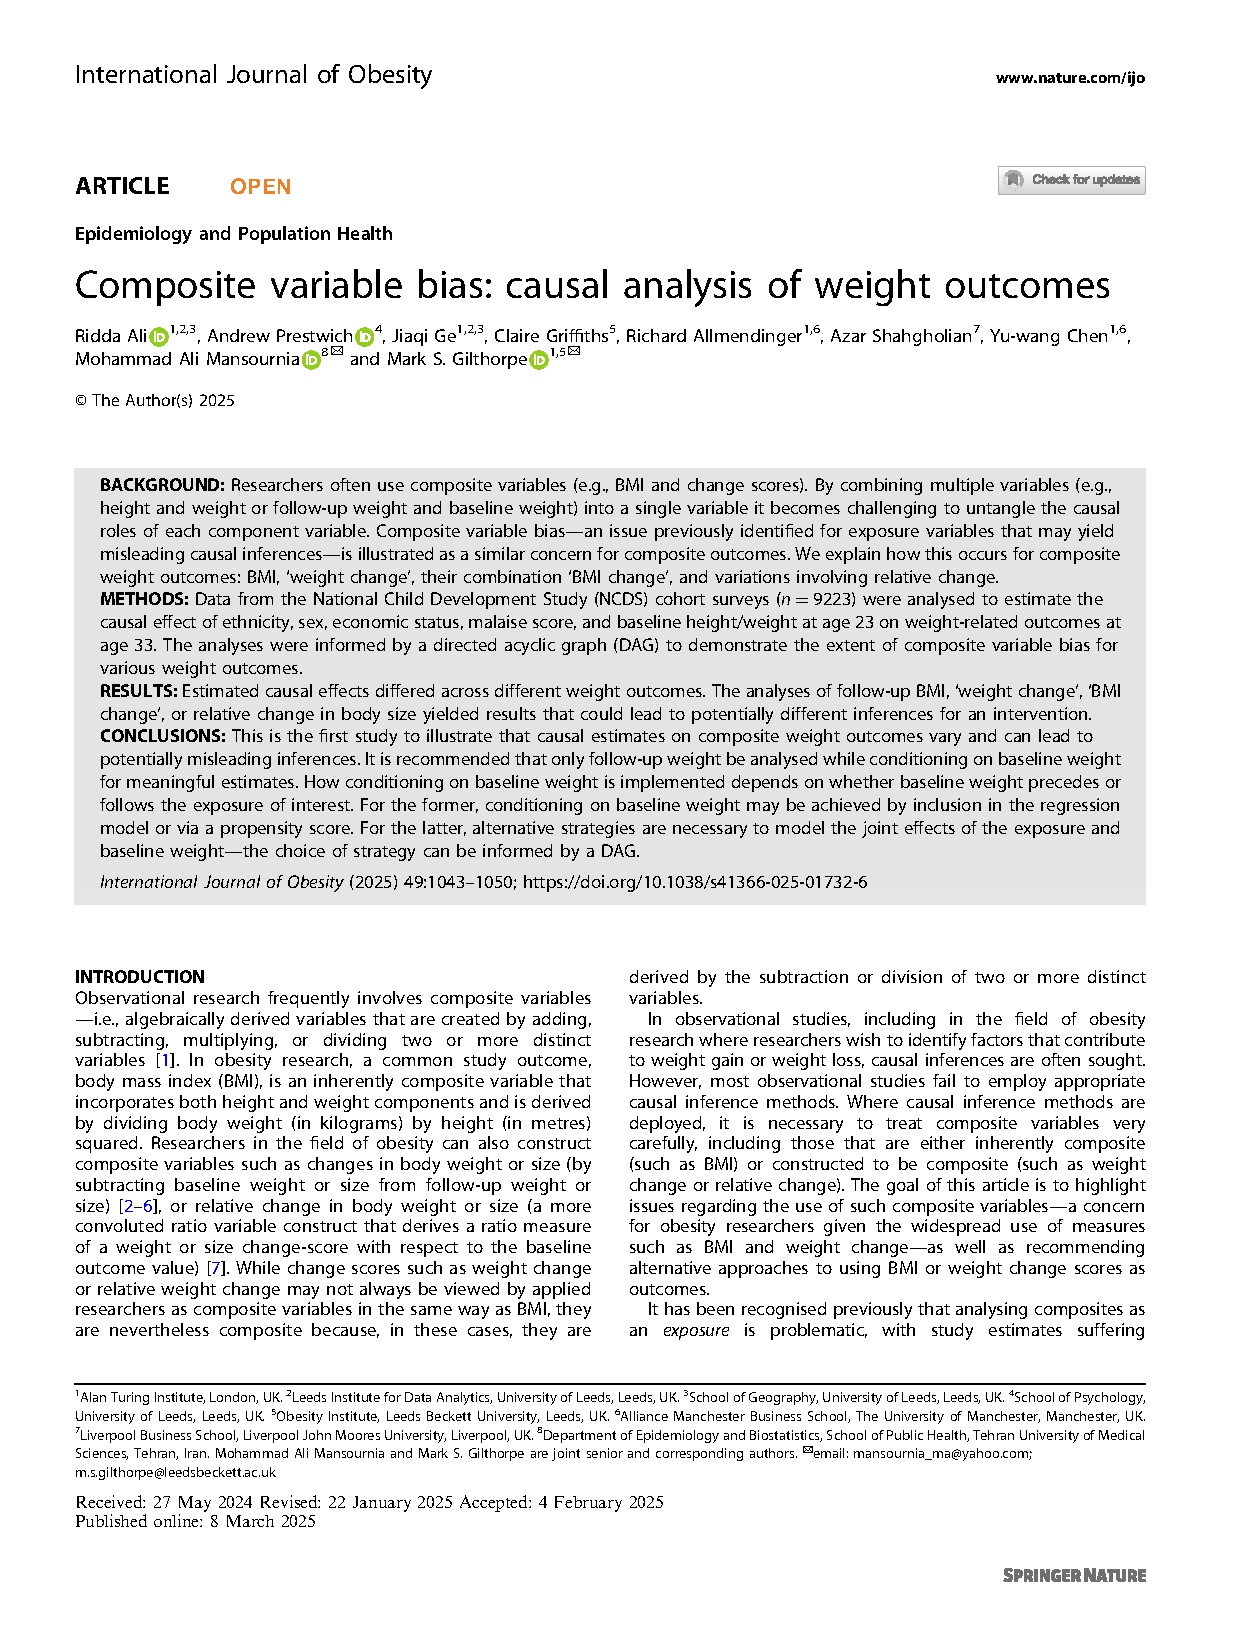
\includepdf[pages=-]{pdfs/10.1038_s41366-025-01732-6.pdf}

\chapter{Modelling emergent pedestrian evacuation behaviors from intelligent, game-playing agents}

\noindent\textbf{Citation:} Y Wang; J Ge; A Comber. (2025) Modelling emergent pedestrian evacuation behaviors from intelligent, game-playing agents. \textit{Journal of Computational Social Science}, 8(2). https://doi.org/10.1007/s42001-025-00369-9

\noindent\textbf{Abstract}\par
\begin{quote}\small
Abstract Much work has been done to understand complex crowd dynamics and self-organizing behaviors in high-density crowd situations. But most approaches for modelling pedestrian dynamics in emergencies require complex computations, making it difficult to capture multiple individual behaviors within a single model. This paper describes an agent-based model (ABM) that incorporates Bayesian game theory into pedestrian simulations. It assumes that players (agents) are playing a Bayesian game (i.e. games with incomplete information) and adopt strategies based on the anticipated behaviors of others to achieve a Bayesian Nash Equilibrium (BNE). Here, the model agents make decisions based on the possible positions of neighbors in the next time period to maximize their comfort and efficiently achieve their evacuation goal. A series of simulation experiments were undertaken using corridors, bottlenecks, and intersections in simulated evacuation spaces with the characteristics of mass tramping accidents. BNE provides a realistic and efficient approach for modelling complicated pedestrian dynamics with strong applicability. The BNE-informed ABM performance (evacuation times, routes, and behaviors) demonstrates its ability to realistically simulate emergent patterns of evacuation behaviors. The results indicate that agents using game theory reflect the behaviors of individuals with crowds well: BNE agents evacuate effectively at low densities and low blockages but are confounded in situations with few route choices in highly constricted spaces. The BNE-informed model provides a platform to better understand diverse crowd behaviors (e.g. herding and self-organized queuing, etc.) in varied spatial contexts, contributing to the designs of urban public space, evacuation planning, and crowd management.
\end{quote}

\vspace{0.5em}
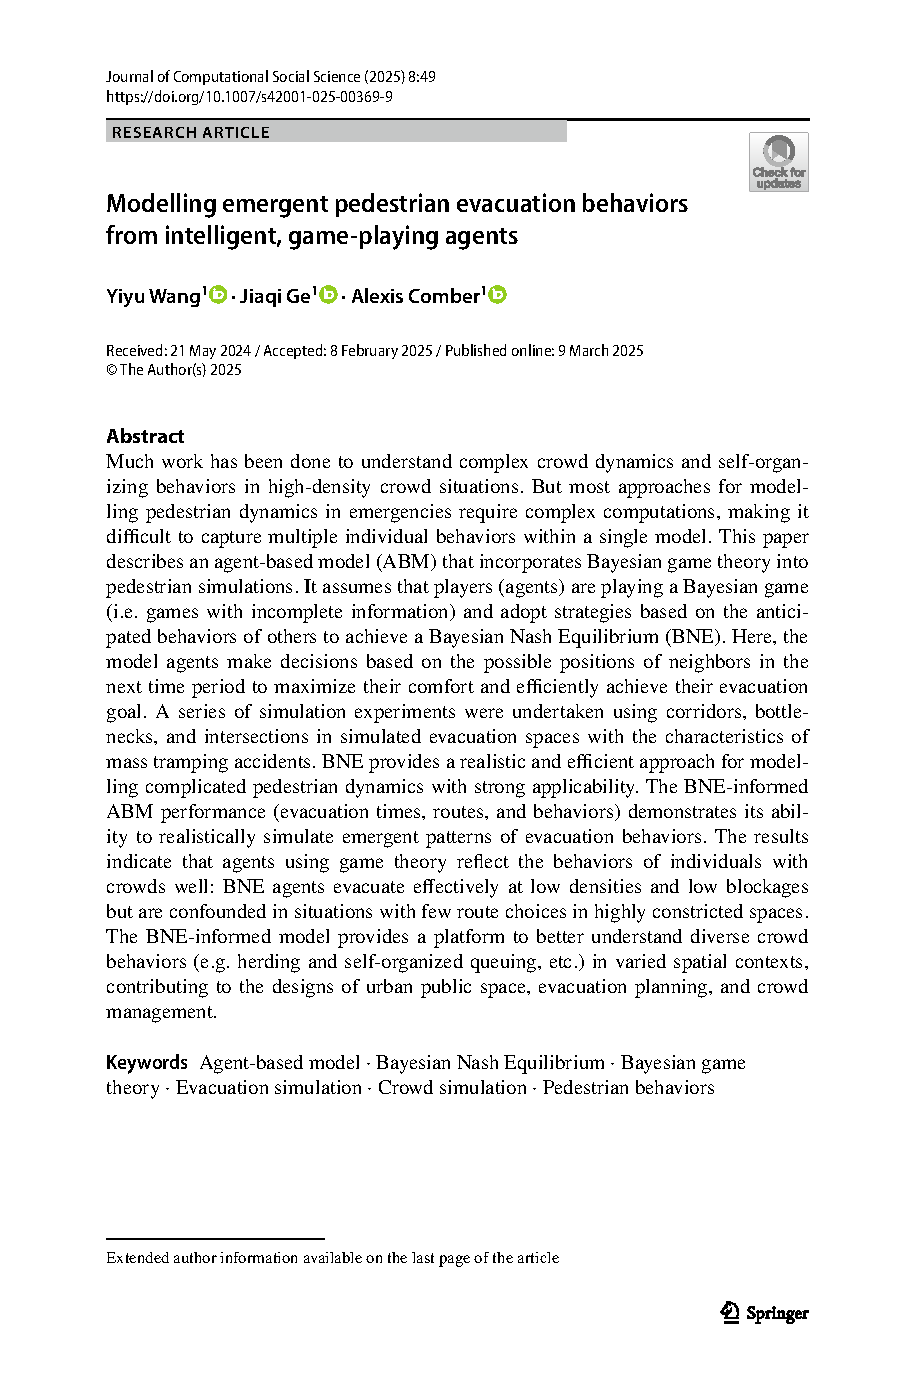
\includepdf[pages=-]{pdfs/10.1007_s42001-025-00369-9.pdf}

\chapter{Investigating the Effectiveness of Station Staff Guidance in Underground Urban Railway Fire Emergencies: Virtual Reality Experiment}

\noindent\textbf{Citation:} Guangxi He; Xiao Li; Yi Zhang; Tao Wang; Bozhezi Peng; Chaoyang Li; Jiaqi Ge; Li Sun; Yingjun Xu. (2026) Investigating the Effectiveness of Station Staff Guidance in Underground Urban Railway Fire Emergencies: Virtual Reality Experiment. \textit{Journal of Transportation Engineering Part A: Systems}, 152(2). https://doi.org/10.1061/jtepbs.teeng-9272

\noindent\textbf{Abstract}\par
\begin{quote}\small
Exploring the critical roles of various factors on determining the wayfinding performance of passengers during a subway fire emergency is important. By developing a virtual reality environment of an underground urban railway station, an immersive virtual reality escape experiment was conducted with a head-mounted device to record the wayfinding performance of 1,151 participants. The experimental data include trajectory data of the participants in the escape task (e.g., time and three-dimensional coordinates) and survey data of personal information. Binary logistic regression, general linear regression, LightGBM, and other methods were employed to analyze the effects of station staffs’ guidance, emergency broadcast, signage, and other factors on wayfinding performance, with station staffs’ guidance being a factor rarely addressed in previous studies. The large sample size enabled the application of ensemble learning methods and facilitated fine-grained group difference analyses that are difficult to achieve in traditional small-sample evacuation experiments. Results show that emergency broadcast and the guidance of station staffs had a highly significant impact on evacuees’ route choice. Education exhibited a positive influence on both evacuees’ route choices and evacuation time. Furthermore, information overload was observed among evacuees under the influence of multiple information sources. The results of this study can not only serve as a theoretical basis for policymakers to understand the determinants of wayfinding performance, but also provide guidance for underground urban railway station or metro station evacuation plan in a fire emergency.
\end{quote}

\vspace{0.5em}
